
\chapter{\textit{$\pi$SOD-M} Environment} 
\label{chap:environment}

\epigraph{``\textit{The computer was born to solve problems that did not exist
before.}''}{Bill Gates}

This chapter describes the $\pi$SOD-M environment for developing reliable
service based systems using the methodology we propose. The $\pi$SOD-M
environment was developed to support the $\pi$SOD-M methodology. The $\pi$SOD-M
based process consists in generating an application starting from a
\textit{$\pi$-UseCase} model and then transforming it into series of models at
the PIM and PSM levels before finally generating the code that implements the
application.
 
%  that implements 
% the generation of {\em Policy} based services' compositions. For a given
% services' based application, the process consists in generating an application
% starting from a $\pi$-UseCase modeling. From a $\pi$-UseCase model,
% transformations between models are made until the platform specific model level
% to generate service composition specification code. Four model to model
% transformations are performed, three transformations between models, and one
% model to text transformation generates the service composition specification in
% $\pi$-PEWS language. All transformations are done through an Eclipse plugin. All
% models definition are the result of a general process defined by the $\pi$SOD-M
% method in which a set of models are built following a service oriented approach. 
 
$\pi$SOD-M environment is built on the top of Eclipse framework
(http://www.eclipse.org), which is a framework to build Integrated Development
Environments (IDEs). We also use the Eclipse
Modelling Framework (EMF), a meta-modelling framework that was devised to be
extended and provides with the utilities needed to define, edit and handle
(meta)-models. To automate the transformation models we use the ATL Language\footnote{ATL uses EMF to handle models (that is to serialize, to navigate and to modify
them). Once the ATL transformation is executed, the ATL engine matches the
source pattern and the source model and instantiates each pattern into the
target model.} \cite{atl_manual}, a model transformation language framed in
Eclipse. Another language used for model transformation is Acceleo \cite{acceleo}, a
model to text engine. $\pi$SOD-M uses this environment~\footnote{\newText{The environmental requirements are the Eclipse Modelling (Galilleo or higher)
and all proposed plugins, \textit{$\pi$-UseCase, $\pi$-ServiceProcess,
$\pi$-SerciveComposition} and \textit{$\pi$-PEWS} editors; and also the
transformation plugins. Because the environment is proposed in the
context of Eclipse, the environmental requirements are also the same needed to
utilize the Eclipse tool.}} to generate service
composition specification code in \textit{$\pi$-PEWS}.

% then for each matching, the target pattern is instantiated in the target model, replacing the match found in the
% source model.

% Thus, ATL works perfectly with the models defined over EMF, as well as
% $\pi$SOD-M plugin. So one, ATL compiler provides features like multiples source
% patterns, rule inheritance, and endpoint rules.



%  After the user model the application and do the
% transformations, as final result, he can have the correspondent code for
% the service application. Thus, the methodology development environment
% is composed of these two platforms (ATL and Acceleo) that assist in the development
% of $\pi$SOD-M based applications.

% It is not necessary the methodology's final user knows Acceleo or ATL
% for modeling an application. These languages have been used only for the
% tools development. The tool's user also does not need have extensive knowledge
% in MDA to use the tool. Knowledge of basic MDA's concepts and what means
% transformation between models are sufficient to adapt and use the tool in a real
% development environment.
 
The remainder of the chapter is organized as follows. Section
\ref{sec:architecture} describes the environment 
architecture, including the definition of meta-models; and, the implementation
of the model transformation process and the code generation engine. In section
\ref{sec:install} describes how to install and use the environment. Section
\ref{sec:extendingEnvironment} describes how to extend the
environment, for adding new components for generation of system specification
in different languages. Section \ref{sec:env_conclusion} concludes the chapter.
 
\section{General Architecture}
\label{sec:architecture}



Figure \ref{fig:policymanager} presents the general architecture for the
$\pi$SOD-M environment and details how components interact with each other. 
Each model has an editor, and transformation tools that support the application
development. 

% This figure
% presents, in general, the same components described in figure
% \ref{fig:environmentComponents}, although emphasizing the context of Eclipse.
% 
% The meta-models and their plugins for editing are at the highest
% level. In an intermediate level we have the ATL based transformation
% components for the models mapping, and finally, the code generation is
% accomplished through the mapping described in Acceleo, generating the
% specification to be executed.
 
\begin{figure} [ht!]   
\centering
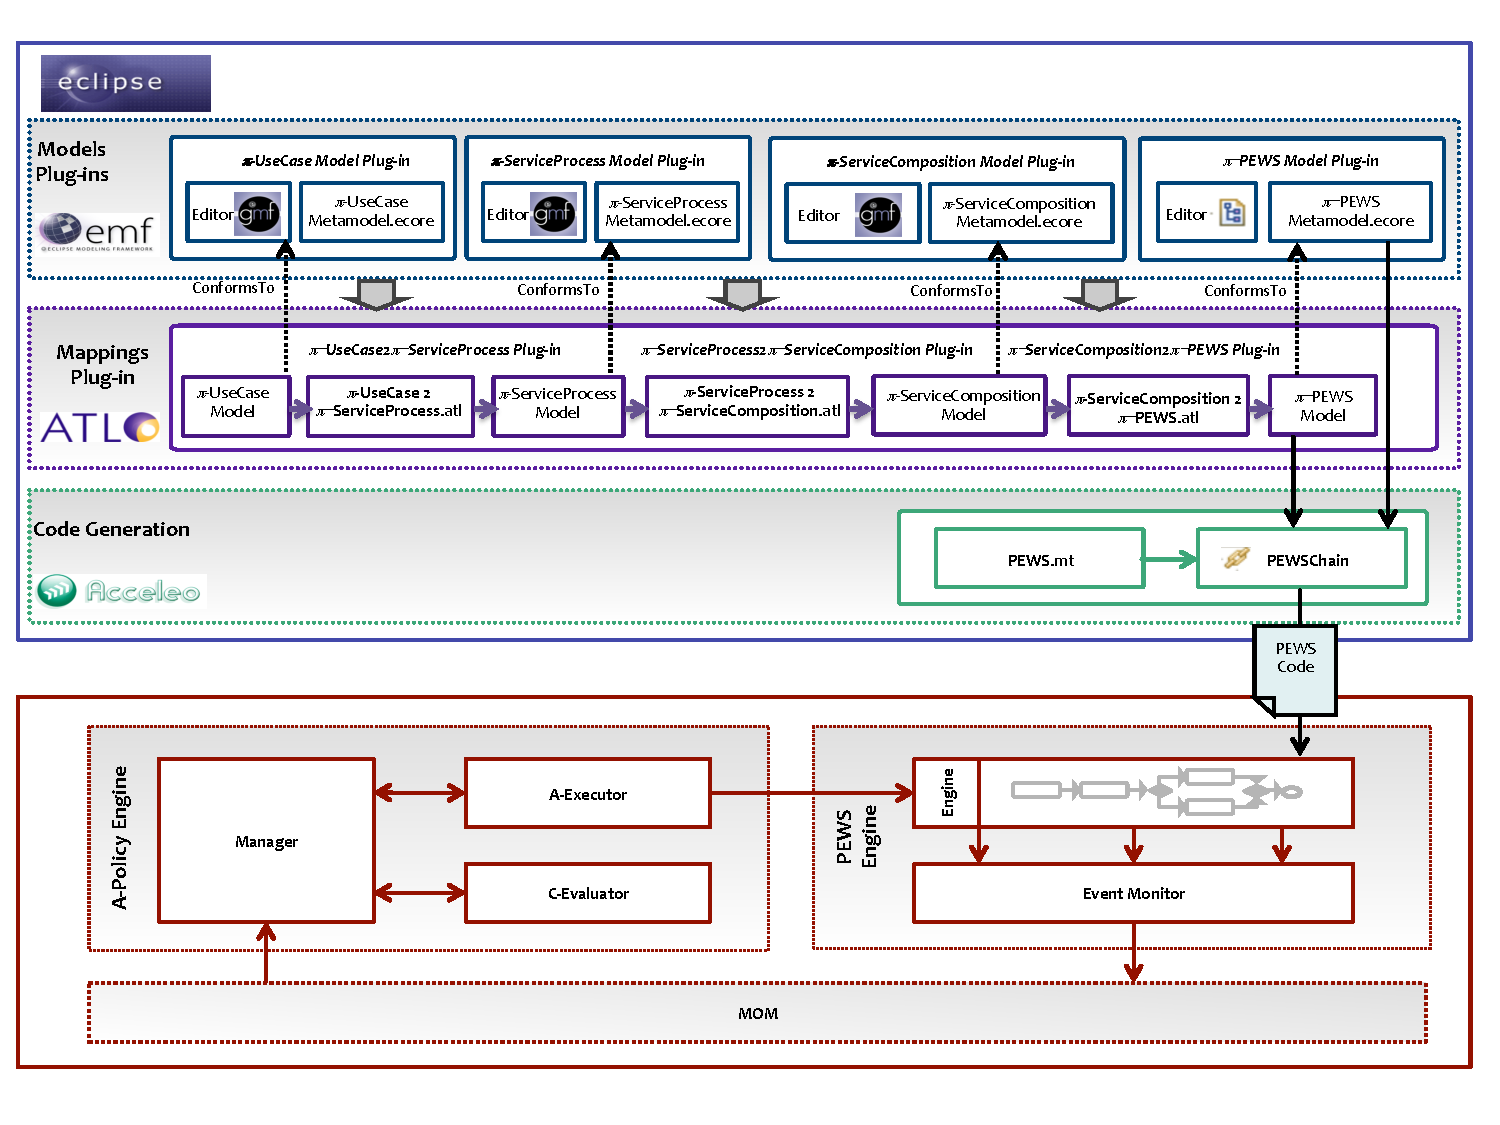
\includegraphics[width=1.0\textwidth]{chapters/methodology/figs/FrameworkOverviewFigure}
\caption{$\pi$SOD-M Development Environment.}
\label{fig:policymanager} 
\end{figure}  

The $\pi$SOD-M environment architecture is organized in
three layers: \textit{(i) Meta-model level, (ii) PIM-to-PIM Transformations
level level, (iii) PIM-to-PSM Transformations level
level} and \textit{(iv)  Code generation level}.
 Each layer comprises a set of components that
together support the $\pi$SOD-M environment. 
This figure presents how those components are implemented by our tool: (i) the
\textit{Meta-model component} (figure \ref{fig:environmentComponents})
represents the \textit{Model plugins module} of figure \ref{fig:policymanager} (together with all methodology
meta-models); (ii) the \textit{PIM-to-PIM Transformations and PIM-to-PSM
Transformations components} (figure \ref{fig:environmentComponents}) represent
the \textit{Mapping plugins module} of figure \ref{fig:policymanager}; 
(iii) the \textit{Code Transformation} component of the figure
\ref{fig:environmentComponents} is implemented by the \textit{Code generation
module} of figure \ref{fig:policymanager}; and (iv) the \textit{Execution
engine} is represented by the lower tier of figure \ref{fig:policymanager}.



% The main components
% are: \textit{(I)} - \textit{$\pi$-UseCase} ecore meta-model,
% \textit{$\pi$-ServiceProcess} ecore meta-model, \textit{$\pi$-ServiceComposition} ecore meta-model and
% \textit{$\pi$-PEWS} ecore meta-model, that are
% sub-components of the \textit{Meta-model component} (\textit{EMF Ecore
% meta-model level}); \textit{(II)} - \textit{$\pi$-UseCase2$\pi$-ServiceProcess} component and
% \textit{$\pi$-ServiceProcess2$\pi$-ServiceComposition} component, that are
% sub-components of the \textit{PIM-to-PIM Transformation component} (\textit{Model transformation
% level}); \textit{(III)} - \textit{$\pi$-ServiceComposition2$\pi$-PEWS}
% component, that are sub-components of the \textit{PIM-to-PSM Transformation
% component}; \textit{(IV)} - the \textit{Code Transformation} component
% (\textit{Code generation level}); and \textit{(V)} - the \textit{Execution Engine} component, comprising both,
% \textit{APolicy Engine} and \textit{PEWS Engine} components. 


 
\begin{figure} [ht!]   
\centering
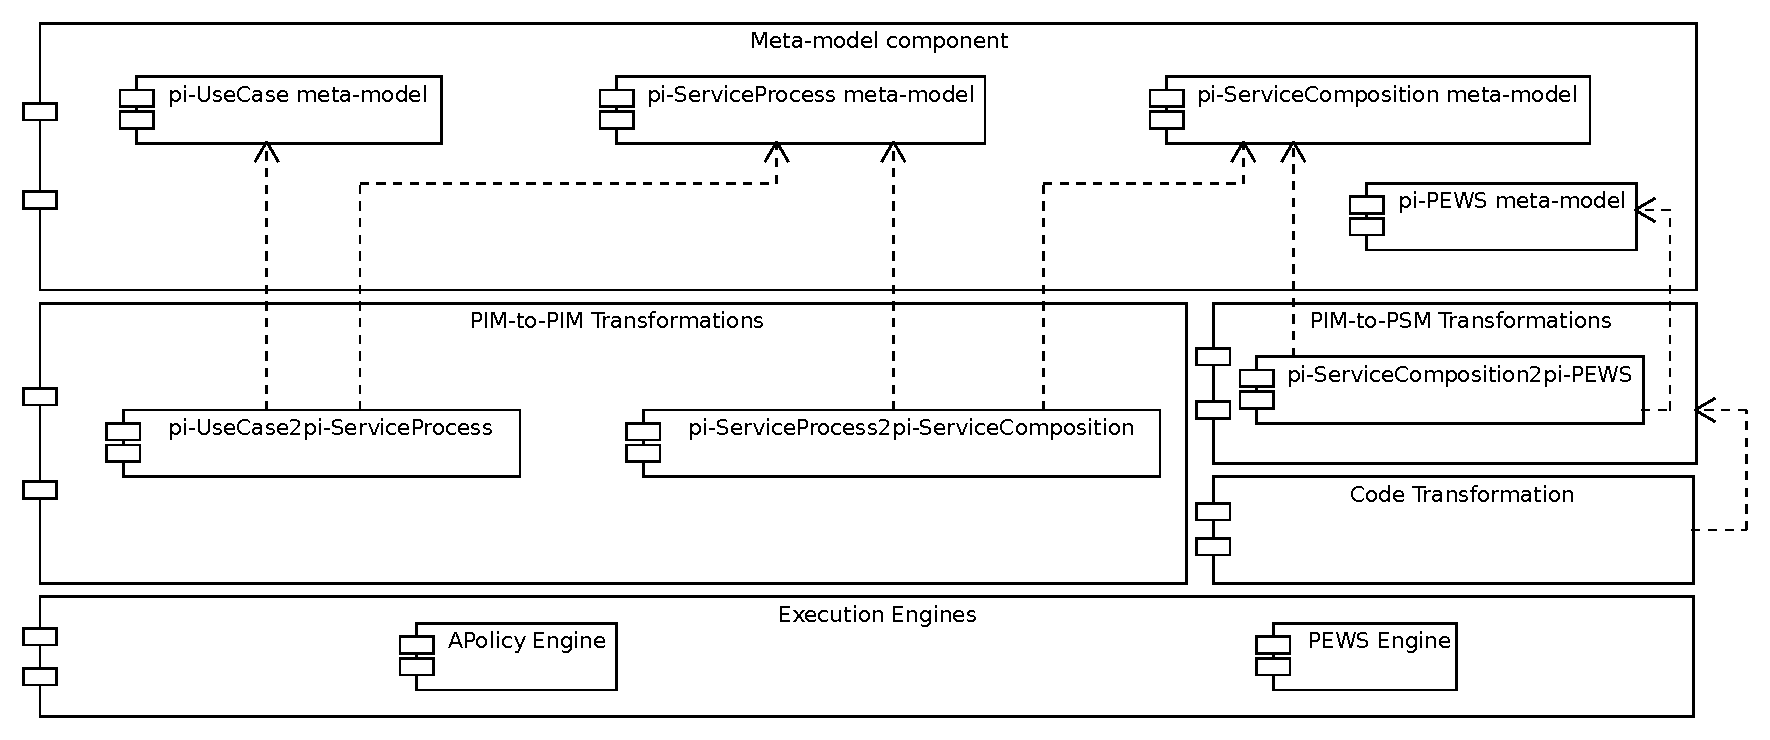
\includegraphics[width=1.0\textwidth]{chapters/implementation/figs/componentsWOE}
\caption{Environment Components.} 
\label{fig:environmentComponents} 
\end{figure} 
  
The \textit{Models plugin module} comprises the components that describe
the $\pi$SOD-M meta-models, and how their models must be created. There are
four meta-model components. All components of the \textit{Mapping plugin module}
depend of the definitions made in \textit{Models plugin}.

When a model transformation is made, the models must comply with their
respective meta-model. The process is executed as follows: every time a
transformation is performed, a consistency check of both, source and target
models is performed. After all transformation are made, the PSM model is
translated into code of a particular platform, in the case of $\pi$SOD-M,
\textit{$\pi$-PEWS} is the chosen platform.  The transformation of PSM model in
code is the last stage of transformation. The component of the \textit{Code
generation module}  depend of the PSM generated by the last model
transformation. Finally, the \textit{Execution Engine} component performs the
execution of the service-based specification code.

 


% The following three sections will detail each particular feature of the
% $\pi$SOD-M development environment.

 
\subsection{Ecore Meta-models (\textit{Models Plugin Module})}

The implementation of each meta-model is defined in \textit{Ecore}\footnote{The 
\textit{Models Plugin Module} is a set of Ecore files that represents all $\pi$SOD-M meta-models. These meta-models are the sources for the development of
each of the methodology's model. All models designed for an application must
obey their meta-model specification. This module is composed by all the proposed
methodology's models in EMF (\textit{.ecore extension}).} files, they are:
\textit{$\pi$-UseCase, $\pi$-ServiceProcess, $\pi$-ServiceComposition} and
\textit{$\pi$-PEWS}.  All meta-models have a related
\textit{genmodel}\footnote{A \textit{.genmodel} is a intermediary file format
used to produce the syntax editor for each meta-model.} definition. The plugin
editor can be created from the \textit{genmodel} definition, so that models can
be specified.  
 
% The Ecore Tools component provides a complete environment to create, edit and
% maintain Ecore models. This component eases handling of Ecore models with a
% Graphical Ecore Editor and bridges to other existing Ecore tools.  
% From a model specification, EMF provides tools and runtime support to produce a
% set of classes for the model, a set of adapter classes that enable viewing and
% command-based editing of the model, and a basic editor. Models can be specified
% using annotated UML, XML documents, or modeling tools, then imported into
% EMF. Most important of all, EMF provides the foundation for interoperability
% with other EMF-based tools and applications. 

% Although there are editors for each model of the methodology, it is still
% necessary components that can make a transformations between them. Thus the
% editing process need not be complete at all levels, but only at the highest
% level, \textit{i.e.} $\pi$-UseCase model, and then make automatic generation for
% the other models.

%After the creation of each meta-model were created their respective plugins.


Using these set of tools (model editors) it is possible to create models
at different $\pi$SOD-M levels. There are editors for all $\pi$SOD-M models:
\textit{$\pi$-UseCase editor, $\pi$-ServiceProcess editor,
$\pi$-ServiceComposition} editor and \textit{$\pi$-PEWS} editor.
  
Although there are editors for each methodology model, it is still
necessary components to perform transformations among them. Thus, the
model specification process can be made in all methodology levels. However it
can be made only at the highest level, \textit{i.e.} \textit{$\pi$-UseCase}
model, and then execute automatic transformation to generate lowest level
models.
 
 \subsection{Model Transformation (\textit{Mapping Plugin Module})}
 
 The \textit{Model transformation level} has a set of components for processing
 and transforming models. The model transformation components are based on
 the source models for generating the equivalent target model. For example, from
 a \textit{$\pi$-UseCase} model is generated the
\textit{$\pi$-ServiceProcess} model, from a \textit{$\pi$-ServiceProcess}
model is generated the \textit{$\pi$-ServiceComposition} model, and finally,
from a \textit{$\pi$-ServiceComposition} model is generated a 
\textit{$\pi$-PEWS} model. After the model generation the
designer can perform refinements. Refinement can improve and adjust elements
that require a more detailed description at this modeling level.
% Figure \ref{fig:policymanager} shows the environment components for the
% processing models transformation. 


$\pi$SOD-M model transformation process is based on the rules described in
chapter \ref{chapter:methodology}. The implementation process requires
additional, more specific information to be taken into account. We had to
consider the representation of our concepts in the Eclipse and ATL environments
for MDA-based application development, \textit{e.g.}, aspects of plugin
generation; design model properties; compliance of the designed
meta-model with the generated model; the specific model implementation; and etc.  


% \begin{itemize}
%   \item Each meta-model is modeled using the EMF environment. During the
%   meta-model definition, a beta plugin version was being generated to verify the
%   model development consistence and coherence. For example the $\pi$-UseCase
%   meta-model, during its definition, short use cases models examples were
%   developed to validate our definition;
%   \item A stable plugin version was generated and then a complete example was
%   modeled to validate the usability of each $\pi$SOD-M model plugin. The
%   sequence of the model plugin development were:
%   \textit{$\pi$-ServiceComposition, $\pi$-PEWS, $\pi$-UseCase} and
%   \textit{$\pi$-ServiceProcess}. We first generated the low level plugins to
%   validate the code generation from a service composition specification.
%   Immediately after we developed the high level model to the complete $\pi$SOD-M
%   support.  
%   \item  With all models well developed and assembled in the tool for each
%   aspect of service model development, it was necessary proceed with the
%   automatic transformation. Each transformation represents, from a specific
%   $\pi$SOD-M model, that it is possible to generate a equivalent lower level
%   $\pi$SOD-M model, \textit{e.g.}, (i) from the $\pi$-UseCase model, the
%   $\pi$-ServiceProcess can be generated; (ii) from the $\pi$-ServiceProcess
%   model a $\pi$-ServiceComposition can be generated; (iii) from the
%   $\pi$-ServiceComposition model, the $\pi$-PEWS model can be generated;  and
%   (iv) from the $\pi$-PEWS model, the system service composition code can be
%   generated.
%   \item By the end, we configure a $\pi$SOD-M Eclipse version for research use.
% \end{itemize}  

We used the Eclipse Modeling Framework (EMF) for implementing the
meta-models  \textit{$\pi$-UseCase, $\pi$-ServiceProcess,
$\pi$-ServiceComposition} and \textit{$\pi$-PEWS}. The ATL language was used
for developing the mapping rules for transformation of models
(\textit{$\pi$-UseCase2$\pi$-ServiceProcess},
\textit{$\pi$-ServiceProcess2$\pi$-ServiceComposition} and
\textit{$\pi$-ServiceComposition2$\pi$-PEWS} plug-ins). 
This plugin takes as input a \textit{$\pi$-PEWS} model implementing a specific
service composition and it generates the code to be executed by the {\em Policy} based
\textit{Execution Engine} (figure \ref{fig:environmentComponents}).

 \begin{figure}  [ht!]
\centering
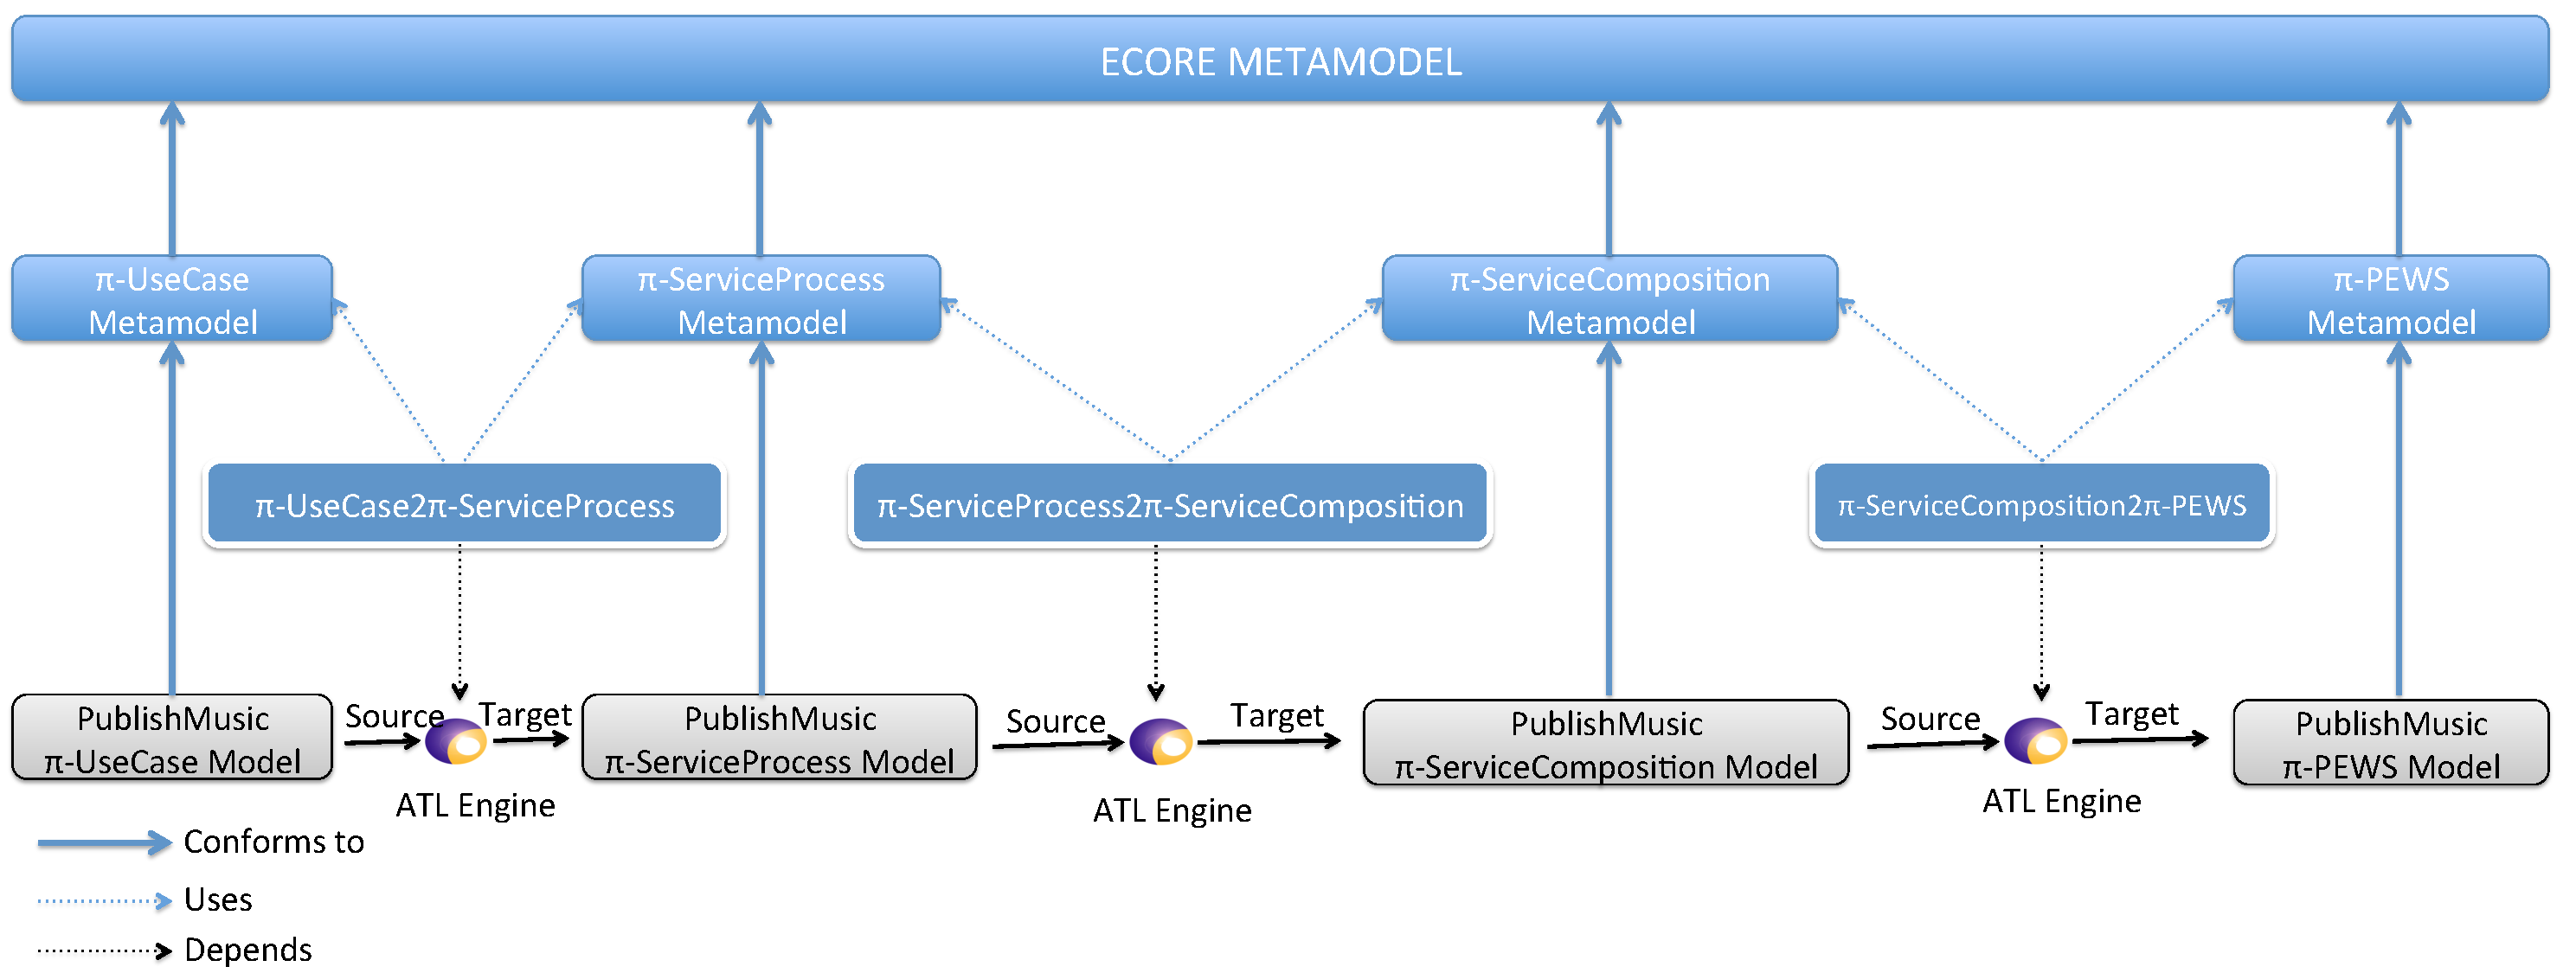
\includegraphics[width=1.0\textwidth]{chapters/methodology/figs/modelTrasformation}
\caption{ATL Model to Model Transformation in $\pi$SOD-M.}
\label{fig:modelTomodelTransfomation}
\end{figure}

 Figures \ref{fig:modelTomodelTransfomation} and 
 \ref{fig:modelToTextTransformation} present a general view of the $\pi$SOD-M
 models transformation, showing the set of plug-ins developed to
 implement it. Figures \ref{fig:modelTomodelTransfomation} presents the
 model-to-model transformations, while figure
 \ref{fig:modelToTextTransformation} shows the model-to-text transformation
 schema. The environment implements the abstract architecture shown in figure
 \ref{fig:policymanager}. This environment consists of plug-ins implementing the
 \textit{$\pi$-UseCase, $\pi$-ServiceProcess, $\pi$-ServiceComposition} and
 \textit{$\pi$-PEWS} meta-models used for defining models; and ATL rules for
 transforming PIM and PSM models (model to model transformation) and finally
 generating code (model to text transformation) with Acceleo.
 
  
\begin{figure} [ht!]  
\centering
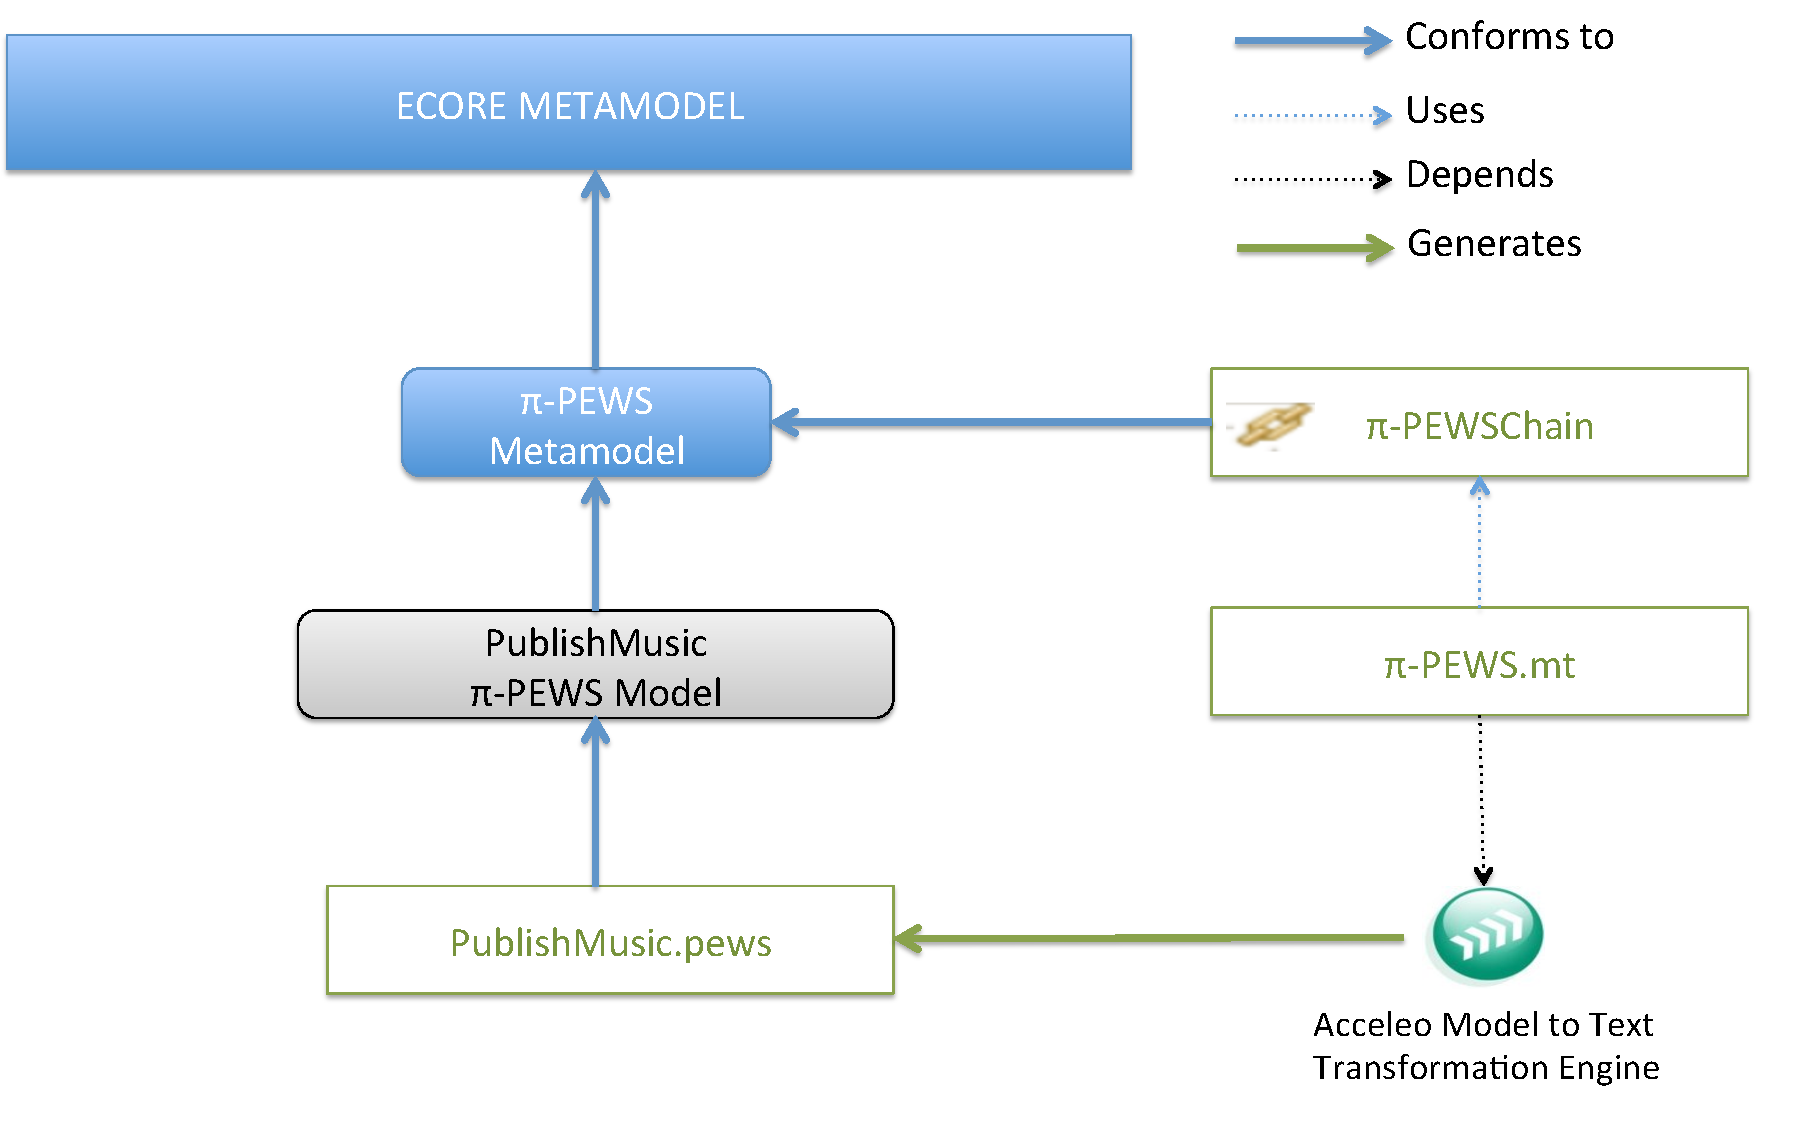
\includegraphics[width=0.7\textwidth]{chapters/methodology/figs/AcceleoTransformationFigure}
\caption{Acceleo Model to Text Transformation in $\pi$SOD-M.}
\label{fig:modelToTextTransformation} 
\end{figure}  


In order to proceed with a model transformation it is necessary to configure the
transformation environment. Figure \ref{fig:configurationATL} presents a
standard screen for configuring each transformation (in this case for the ``to
publish music'' scenario). From any source model, for example,
\textit{$\pi$-UseCase, $\pi$-ServiceProcess} or
\textit{$\pi$-ServiceComposition}, the system can perform the automatic
transformation. Using the transformation tool of figure
\ref{fig:configurationATL} requires from the user: (1) to indicate the
ATL transformation rules file; (2) to choose the source meta-model reference
(.ecore file); (3) to choose the target meta-model reference (.ecore file); (4) 
to choose the source model that will be transformed (\textit{e.g.
music.piusecase} file); (5) to choose the target model that will be generated
(\textit{e.g. music.piserviceprocess} file); and finally, (6) to run the tool.
The same must be performed for all model-to-model transformations. For model-to-text
transformation, the rule file to be chosen should be the
Acceleo file.
 

\begin{figure}[ht!]
\centering
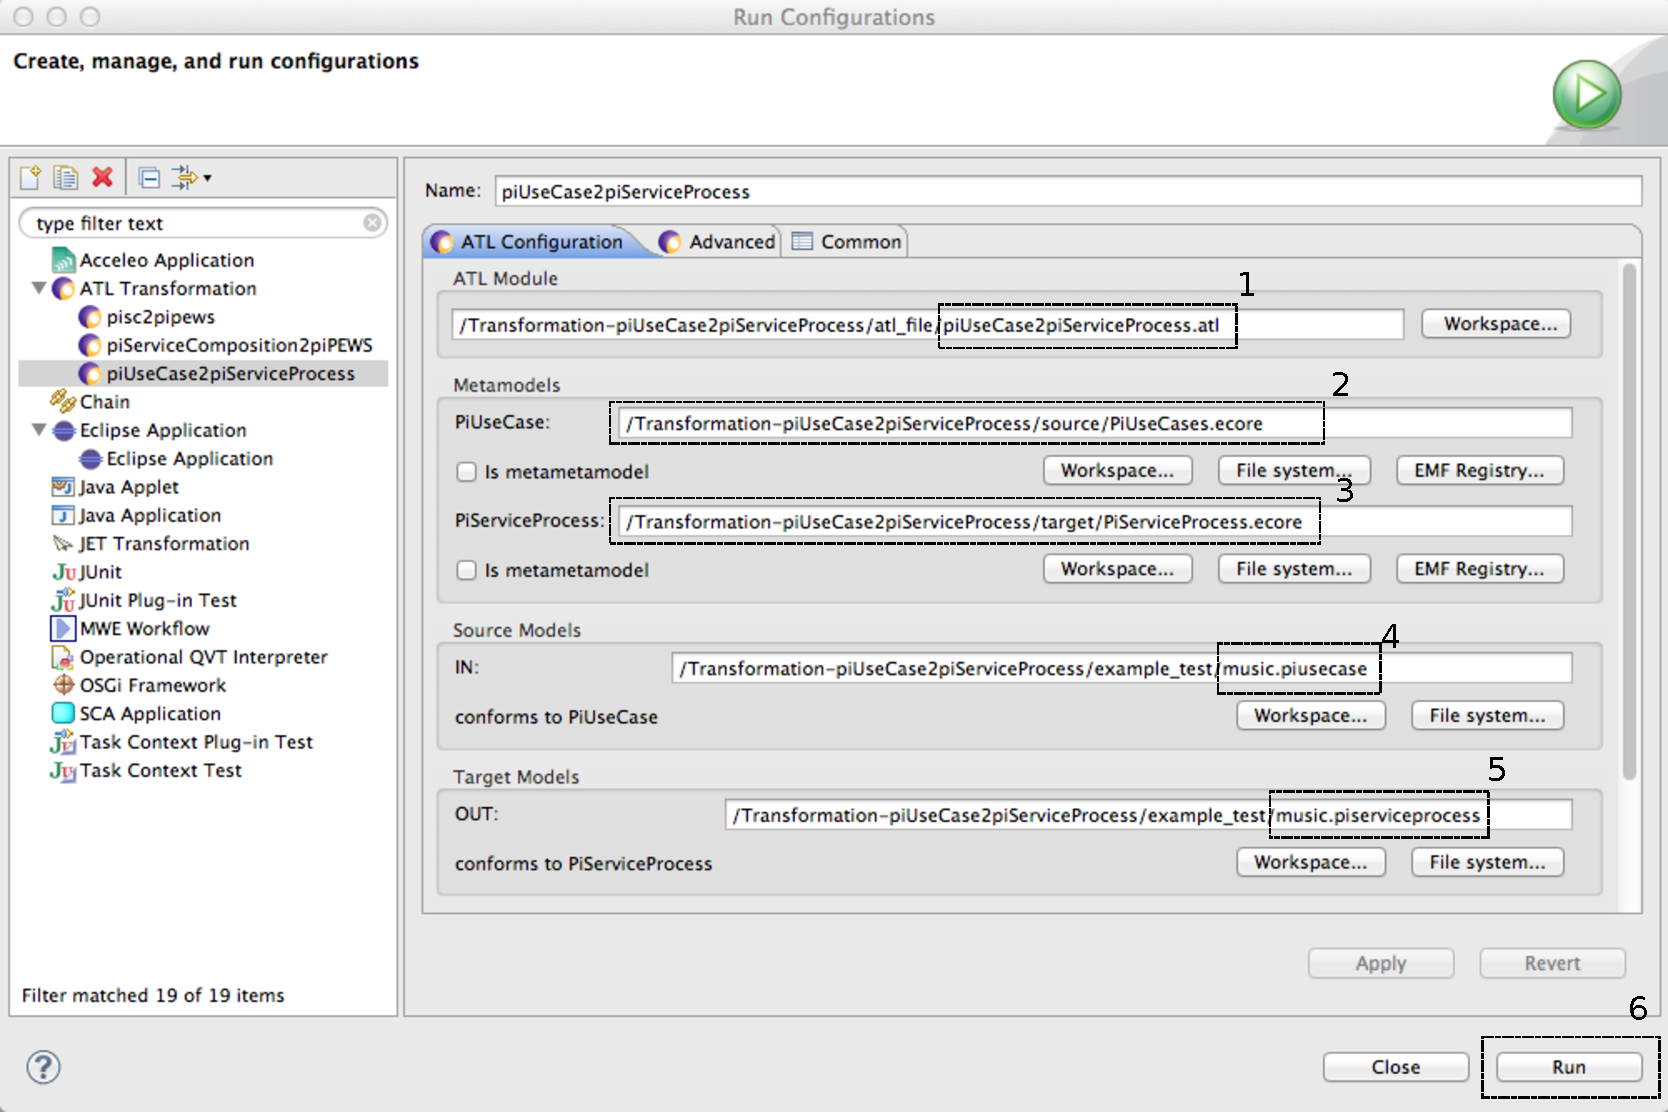
\includegraphics[width=.90\textwidth]{chapters/implementation/figs/ATL-trasnformationPiUseCase2PiServiceProcess.pdf}
\caption{ATL Configuration for $\pi$SOD-M Transformation.}
\label{fig:configurationATL}
\end{figure}


As an example, figure \ref{fig:configurationATL} shows the configuration for the
transformation from \textit{$\pi$-UseCase} (source) to
\textit{$\pi$-ServiceProcess} (target). Notice that, in this case, the reference
meta-models must be the same. For further transformations, this process must
follow the same sequence, changing only the models and reference meta-models.

\subsubsection{\textit{$\pi$-UseCase2$\pi$ServiceProcess} Transformation Rules}

The transformation rules describe how models are transformed. As a general rule, 
the automatic transformation of models favors a faster development of
applications. In most cased, the environment or the designer should verify if
the transformations are valid or not. In the $\pi$SOD-M environment, the
consistency of the transformations must be performed by the designer. If a
problem on the transformation is identified, the target model can be modified manually.


\begin{figure}
\tiny
\centering

\begin{lstlisting}[label=list:exampleRules,caption=ATL Example Rule.]

1  rule ruleName{	 
2	  from		
3		  var_sourceName: SourceModel!Entity
4	  to
5		  var_targetName: TargetModel!Entity(
6			  atribute_1 <- var_sourceName.atribute_a,
7			  atribute_2 <- var_sourceName.atribute_b	
8		  )
9  }
\end{lstlisting}
\label{fig:exampleRule} 
\end{figure}   


In ATL, there exist two different kinds of rules that correspond to the two
different programming modes provided by ATL (e.g. declarative and imperative
programming). The \textit{matched rules}\footnote{The matched rules constitute
the core of an ATL declarative transformation since they make it possible to
specify 1) for which kinds of source elements target elements must be generated,
and 2) the way the generated target elements have to be initialized. A matched
rule is identified by its name. It matches a given type of source model element,
and generates one or more kinds of target model elements. The rule specifies the
way generated target model elements must be initialized from each matched source
model element\cite{atl_manual}.}  (declarative programming) and the
\textit{called rules}\footnote{The called rules provide ATL developers with convenient
imperative programming facilities. Called rules can be seen as a particular type
of helpers: they have to be explicitly called to be executed and they can accept
parameters. However, as opposed to helpers, called rules can generate target
model elements as matched rules do. A called rule has to be called from an
imperative code section, either from a match rule or another called
rule\cite{atl_manual}.} (imperative programming) \cite{atl_manual}. For the $\pi$SOD-M environment, we
use both types of rules. Listing \ref{list:exampleRules} shows a general example of an
ATL \textit{matched rule}. According to this, we will present the main ATL rules used to
implement the model transformation. As described in listing
\ref{list:exampleRules}, a rule consists of a name (line 1), a source entity
(\textit{from} clause in lines 2-3), and one or more target entities (\textit{to} clause in line 4-5). Each entity has a name, such as \textit{var\_sourceName} and
\textit{var\_targetName}. The transformation is performed by each entity
attribute and general rules established in each case.


% The rules for automatic \textit{$\pi$-UseCase2$\pi$ServiceProcess}
% transformation comply with the description made in section
% \ref{sec:models-tranformation}, and we present some rules in ATL for model
% transformation in $\pi$SOD-M. 





\begin{figure}
\tiny
\centering

\begin{lstlisting}[label=list:useCase2Action,caption=ATL -
piUseCase2piServiceProcess : useCase2action Rule. ]

1  rule useCase2action {
2  	 from usecase : PiUseCase!FunctionalBasicUseCase(		
3   	 usecase.extend->size() >= 2	
4  	 )
5  	 to sp_action :  PiServiceProcess!Action (
6		  name <- usecase.name
7	 ), sp_serviceActivity : PiServiceProcess!ServiceActivity(
8		 action <- sp_action,
9		 name <- usecase.name + 'SA',
10		 serviceProcess <- thisModule.raiz_piUseCase
11	 ), sp_contract: PiServiceProcess!Contract(					
12		 name <- usecase.name + 'Contract',
13		 assertionInContract <- usecase.UCContraint,
14		 action <- sp_action,
15		 serviceProcess <- thisModule.raiz_piUseCase
16	 ) 	
17 }
\end{lstlisting}
%\label{fig:pewscontract} 
\end{figure}   


\begin{figure}
\tiny
\centering

\begin{lstlisting}[label=list:constraint2contract,caption=ATL -
piUseCase2piServiceProcess : constraint2contract Rule. ]

1  rule constraint2contract{	 
2	  from		
3		  constraint: PiUseCase!UseCaseConstraint
4	  to
5		  assertion: PiServiceProcess!Assertion(
6			  name <- constraint.name,
7			  description <- constraint.description	
8		  )
9  }
\end{lstlisting}
%\label{fig:pewscontract} 
\end{figure}   

Listing \ref{list:useCase2Action} shows the ATL transformation rule between a
{\sc Use Case} and an {\sc Action}, while listing \ref{list:constraint2contract}
shows the transformation rule between {\sc Constraint} and {\sc Assertion}.
There is a restriction in the rule presented in listing
\ref{list:useCase2Action} (line 3), which defines that there must be more than
two {\sc Extend} relation between use cases. In this case, all use cases are
transformed into actions, and are grouped into a {\sc Service Activity} (lines
7-10). And all the constraints are transformed in a set of assertions that are
automatically associated with a {\sc Contract} (lines 11-15). This
transformation (listing \ref{list:useCase2Action}) describes that from a {\sc
Use Case} (lines 2), {\sc Actions}, {\sc Service Activity} and {\sc Contract}
can be generated (lines 5, 7 and 11). It depends on the existence of {\sc
Constraint} or dependence elements ({\sc Incllude} or {\sc Extend}) related to
this use case (line 3).

The listing \ref{list:constraint2contract} describes that all {\sc Constraint}
(\textit{from} clause in lines 2-3) are directly transformed into an
{\sc Assertion} (\textit{to} clause in lines 4-5) (there is no restriction in
the this clause). The restrictions are treated in separate rules such as in
listing \ref{list:useCase2Action}. 



\subsubsection{\textit{$\pi$-ServiceProcess2$\pi$-ServiceComposition}
Transformation Rules} 

As the \textit{$\pi$-ServiceComposition} model is a
refinement of some concepts defined in \textit{$\pi$-ServiceProcess}, such as 
{\sc Contract} and {\sc Activity Services}, most of the transformation
between these models are through direct transformation, without restrictions.
We present the ATL transformation (listing
\ref{list:rooServiceProcess2rootServiceComposition}) of the root element that
comprises the main elements of both models.


\begin{figure}
\tiny
\centering

\begin{lstlisting}[label=list:rooServiceProcess2rootServiceComposition,caption=ATL -
piServiceProcess2piServiceComposition : root Rule. ]

1  rule root {
2 	from		
3 		root: piServiceProcess!ServiceProcess
4	to
5		root_service: piServiceComposition!CompositionServiceModel(
6			activities <- root.activity,
7			edges <- root.edge,
8			compositionPolices <- root.contract
9		)
10 }

\end{lstlisting} 
\label{fig:pewscontract} 
\end{figure}

Listing \ref{list:rooServiceProcess2rootServiceComposition} shows the
transformation rule for the main elements from \textit{$\pi$-ServiceProcess} 
to \textit{$\pi$-ServiceComposition} model. The {\sc Activities} and its
{\sc Edges}, and {\sc Contracts}, which are transformed into {\sc Policy} (lines
6-8). Other rules that describe the transformation between {\sc Assertions} into
policy {\sc Rule} are other type of transformation. However, other rules
describe that all {\sc Contracts} must belong to a specific {\sc Non-functional
Requirement}, for example, all contracts for the performance restrictions, will
be grouped into a single  performance {\sc Policy}. This listing is an ATL
example for \textit{$\pi$-ServiceProcess} model transformation into 
to \textit{$\pi$-ServiceComposition} model.

\subsubsection{\textit{$\pi$-ServiceComposition2$\pi$-PEWS} Transformation
Rules}

The transformation \textit{$\pi$-ServiceComposition2$\pi$-PEWS} is
unique among PIM and PSM levels, however there is no difference in the
rules description in ATL, since all rules are defined in terms of
meta-models rather than specific models. Thus, PIM-to-PSM transformation rules
in ATL follow the same syntax and semantics of the PIM-to-PIM transformation
rules.

The model to be generated in this transformation, namely \textit{$\pi$-PEWS}
model, will be used as input for the code generation component, so that the
application code specification is generated. The listings \ref{list:rootSC2PEWS} and \ref{list:rulePre} present two
transformation rules in ATL. The first describes the transformations of the main
elements for the description of a service composition, the main path, the name
of the specification, the services and policies (lines 6 - 9), while
listing \ref{list:rulePre} describes a policy {\sc Rule} and its related concepts, such as
{\sc Action}, {\sc Event} and {\sc Condition}. The ATL rule has a constraint
to be checked (line 4), what kind of {\sc Rule} is being translated for the
specific language, because depending on the type, the transformation will be
change. The {\sc Rule} element (line 15) consists of all the properties necessary to
create a {\sc Pre-condition}, such as {\sc Action}, {\sc Event} and {\sc Condition} (lines 16-18),
and to which {\sc Policy} the {\sc Pre-condition} is related (line 19).


\begin{figure} 
\tiny
\centering

\begin{lstlisting}[label=list:rootSC2PEWS,caption=ATL -
piServiceComposition2piPEWS : root Rule. ]

1  rule root{ 
2	 from sCM : pisc!CompositionServiceModel
3	 to 
4	 	path: pipews!Path (),
5	 	pews : pipews!PEWSCTSpec (
6			name <- 'newModelPEWSpecName',
7			has <- path,
8			contains <- sCM.partition,
9			defines <- 	thisModule.policies
10		)
11  }
\end{lstlisting}
\label{fig:pewscontract} 
\end{figure}   
\begin{figure}
\tiny
\centering

\begin{lstlisting}[label=list:rulePre,caption=ATL -
piServiceComposition2piPEWS : Pre-condition Rule. ]

1  rule rulePre{
2 	 from
3		r: pisc!Rule (
4			r.event = #PRE)
5	 to
6		rAct: pipews!Action(
7			act <- r.action
8		),
9		rEvt: pipews!Event( 
10			type <- #ActivityPrepered
11		),
12		rCond: pipews!Condition(
13			expression <- r.condition
14		),
15		rRule: pipews!Precondition(			
16			calls <- rAct,
17			defines <- rCond,
18			hasSome <- rEvt,
19			policy <- r.policy
20		)
21  }

\end{lstlisting}
\label{fig:pewscontract} 
\end{figure}



% The next section will show how the code is generated from a \textit{$\pi$-PEWS}
% model.

\subsection{Code Generation  (\textit{Code Generation Module})}
 }
 
\newText{ 
 The $\pi$SOD-M methodology and its environment use $\pi$-PEWS\footnote{Other meta-models and
 transformations can be defined for supporting  code generation into WS-BPEL,
 XAML and other languages adapted for describing business/service process.} as
 intermediate language for supporting the generation of executable code. 
 $\pi$-PEWS is a behavioral language for defining web services interfaces by
 specifying the input/output interface of a web service exported method but also
 the expected behaviour of its methods (e.g., dependencies, exchanged messages).
 The extension  $\pi$-PEWS extension was inspired by languages like JCML
 \cite{CostaMMN12}, JML \cite{LeavensKP07} and Eiffel \cite{Meyer92b}, which
 introduce the notion of  contract for specifying the behavior of a function. In
 $\pi$-PEWS this behaviour can be specified by defining the order in which the
 methods of  services will be executed within a business process and methods
 input/output restrictions. 
 }
 
The $\pi$SOD-M architecture's code generation component (\textit{\textit{Code
generation level}}) is a \textit{$\pi$-PEWS} specification generator. The
code is produced from a \textit{$\pi$-PEWS} model, after it be generated by a
model transformation from \textit{$\pi$-ServiceComposition} model. This
component was implemented using Acceleo \cite{acceleo}. Figure
\ref{fig:sequenceDiagram} presents a sequence diagram describing the model
transformation process and how the designer interacts with the environment to
specify each $\pi$SOD-M model until the specification code is generated.


\begin{figure}[ht!]
\centering
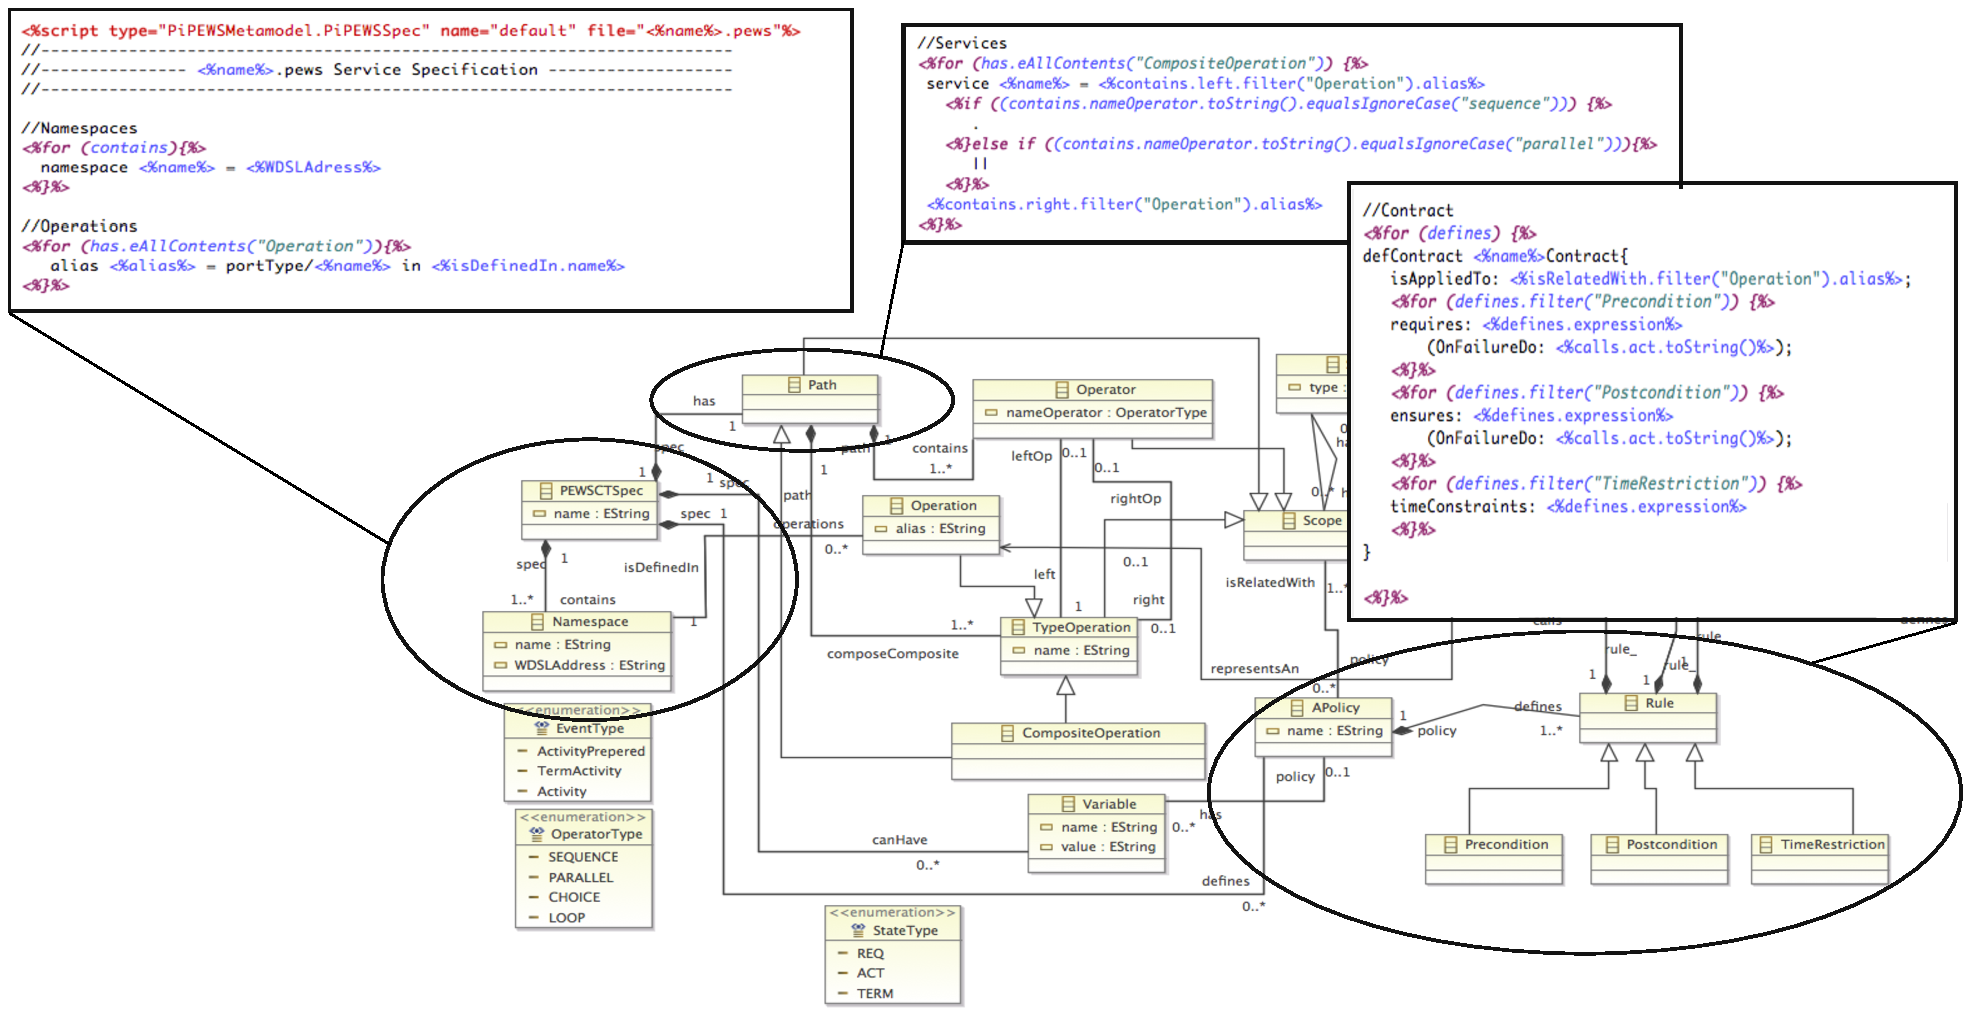
\includegraphics[width=1.0\textwidth]{chapters/implementation/figs/codeGeneration.pdf}
\caption{Acceleo Specification for \textit{$\pi$-PEWS} Code Generation.}
\label{fig:acceleoCode}
\end{figure}



Figure \ref{fig:acceleoCode} presents the \textit{$\pi$-PEWS} meta-model
developed using EMF and some pieces of Acceleo specification. This figure shows
the specification for the \textit{Namescape, Operation, Service} and
\textit{Contract} code generation for \textit{$\pi$-PEWS}. After the code
transformation process, a \textit{.pews} file is created. The listing
\ref{list:namespace}, \ref{list:service} and \ref{list:contract} present parts of Acceleo code for the \textit{$\pi$-PEWS} code generation. The code are the same presented in figure
\ref{fig:acceleoCode}, which presents the relation between the meta-model
concepts and the Acceleo code. The code generation follow the language syntax
described in appendix \ref{append:pews_language}.


     
\begin{figure}
\tiny
\centering

\begin{lstlisting}[label=list:namespace,caption=Acceleo - Namespace and
Operation Code Specification.] 
1  <%script type="PiPEWSMetamodel.PEWSSpec" name="default"
2  file="<%name%>.pews"%>
3  //-----------------------------------------------------------------
4  //------------ <%name%>.pews Service Specification ----------------
5  //-----------------------------------------------------------------

7  //Namespaces
8  <%for (contains){%>
9    namespace <%name%> = <%WDSLAdress%>
10  <%}%>

12  //Operations
13  <%for (has.eAllContents("Operation")){%>
14    alias <%alias%> = portType/<%name%> in <%isDefinedIn.name%> 
15  <%}%>
\end{lstlisting}
\label{fig:pewscontract} 
\end{figure}   


In listing \ref{list:namespace} (lines 1-2) references the 
meta-model, the root element (\textit{PEWSSpec}), and the
name of the generated file (\textit{<\%name\%>.pews}). Lines 3-5 presents the
name of the service specification. Lines 7-10 describes a \textit{for}
integration in the \textit{contains} relationship between \textit{PEWSSpec} and
\textit{Namespace}, and lines 12-15 all operations defined in each
\textit{Namespace} is generated. This operations came from the
\textit{isDefinedIn} relationship between \textit{Namespace} and
\textit{Operation} entities.

\begin{figure}
\tiny
\centering

\begin{lstlisting}[label=list:service,caption=Acceleo - Service Code
Specification.] 
1   //Services
2   <%for (has.eAllContents("CompositeOperation")) {%>	
3     service <%name%> = <%contains.left.filter("Operation").alias%> 
4     <%if ((contains.nameOperator.toString().equalsIgnoreCase("sequence"))) else if((contains.nameOperator.toString().equalsIgnoreCase("parallel")))%> 
9    <%contains.right.filter("Operation").alias%>
10  <%}%>
\end{lstlisting}
\label{fig:pewscontract} 
\end{figure}     

Listing \ref{list:service} presents the Acceleo specification for the
\textit{$\pi$-PEWS} model transformation into code. A service is an alias for
one or more operations. Listing \ref{list:contract} specifies the contract generation, using the
\textit{defines} relationship between \textit{APolicy} and \textit{Rule}. Each
contract have a set of rules for the specification. 
 
\begin{figure}
\tiny
\centering

\begin{lstlisting}[label=list:contract,caption=Acceleo - PEWS Contract
Code Specification.] <%script type="PEWSMetamodel.PEWSCTSpec" 
1  //Contract
2  <%for (defines) {%>	
3  defContract <%name%>Contract{
4	 isAppliedTo: <%isRelatedWith.filter("Operation").alias%>;
5	 <%for (defines.filter("Precondition")) {%>
6	 requires: <%defines.expression%>
7  		(OnFailureDo: <%calls.act.toString()%>);
8	 <%}%>
9	 <%for (defines.filter("Postcondition")) {%>
10	 ensures: <%defines.expression%>
11 		(OnFailureDo: <%calls.act.toString()%>); 
12	 <%}%>
13	 <%for (defines.filter("TimeRestriction")) {%>
14	 timeConstraints: <%defines.expression%>
15	 <%}%>
16 }	
	
 <%}%>
\end{lstlisting}
\label{fig:pewscontract} 
\end{figure}   


The generated code can be executed in both, \textit{$\pi$-PEWS}
and A-Policy engines\footnote{ Both engines are currently under development. The
\textit{$\pi$-PEWS} engine is being developed at UFRN anf the A-Policy engine in
being developed at Grenoble/France.}  These 2 engines are not native components
in the $\pi$SOD-M plugin. The environment supports the process design to
generate code in any language. New language editor components, like BPEL or XAML, can be easily
coupled to the environment. Therewith, it is necessary to add the language
meta-model and make the transformation process. Thus, from a
\textit{$\pi$-ServiceComposition} model, different models and codes can be
generated (not only \textit{$\pi$-PEWS}). This requires only the definition of
equivalent meta-models, and the corresponding code transformation rules.
 
The composition engine manages the life cycle of the composition. Once a
composition instance is activated, the engine schedules the composition
activities according to the composition control flow. Each activity is seen as
a process where the service method call is executed. The execution of an
activity has four states: prepared, started, terminated, and failure. The
execution of the control flow (sequence, and/or split and join) can also be
prepared, started, terminated and raise a failure.



At execution time, the evaluation of policies done by the {\sc Policy} manager
must be synchronized with the execution of the services composition (i.e., the
execution of an activity or a control flow).  Policies associated to a scope are
activated when the execution of its scope starts. A {\sc Policy} will have to
be executed only if one or several of its rules is triggered. If several rules
are triggered, the {\em Policy} manager first builds an execution plan that
specifies the order in which such rules will be executed according to the
strategies defined in the following section.        
%Once rules have been executed, the {\em A-policy} finishes its execution and returns to a sleeping state.
If rules belonging to several policies are triggered then policies are also
ordered according to an execution plan. The execution of policies is out of the
scope of this thesis, the interested reader can refer to
\cite{Espinosa-Oviedo2011a} for further details. 



\begin{landscape}
\begin{figure}
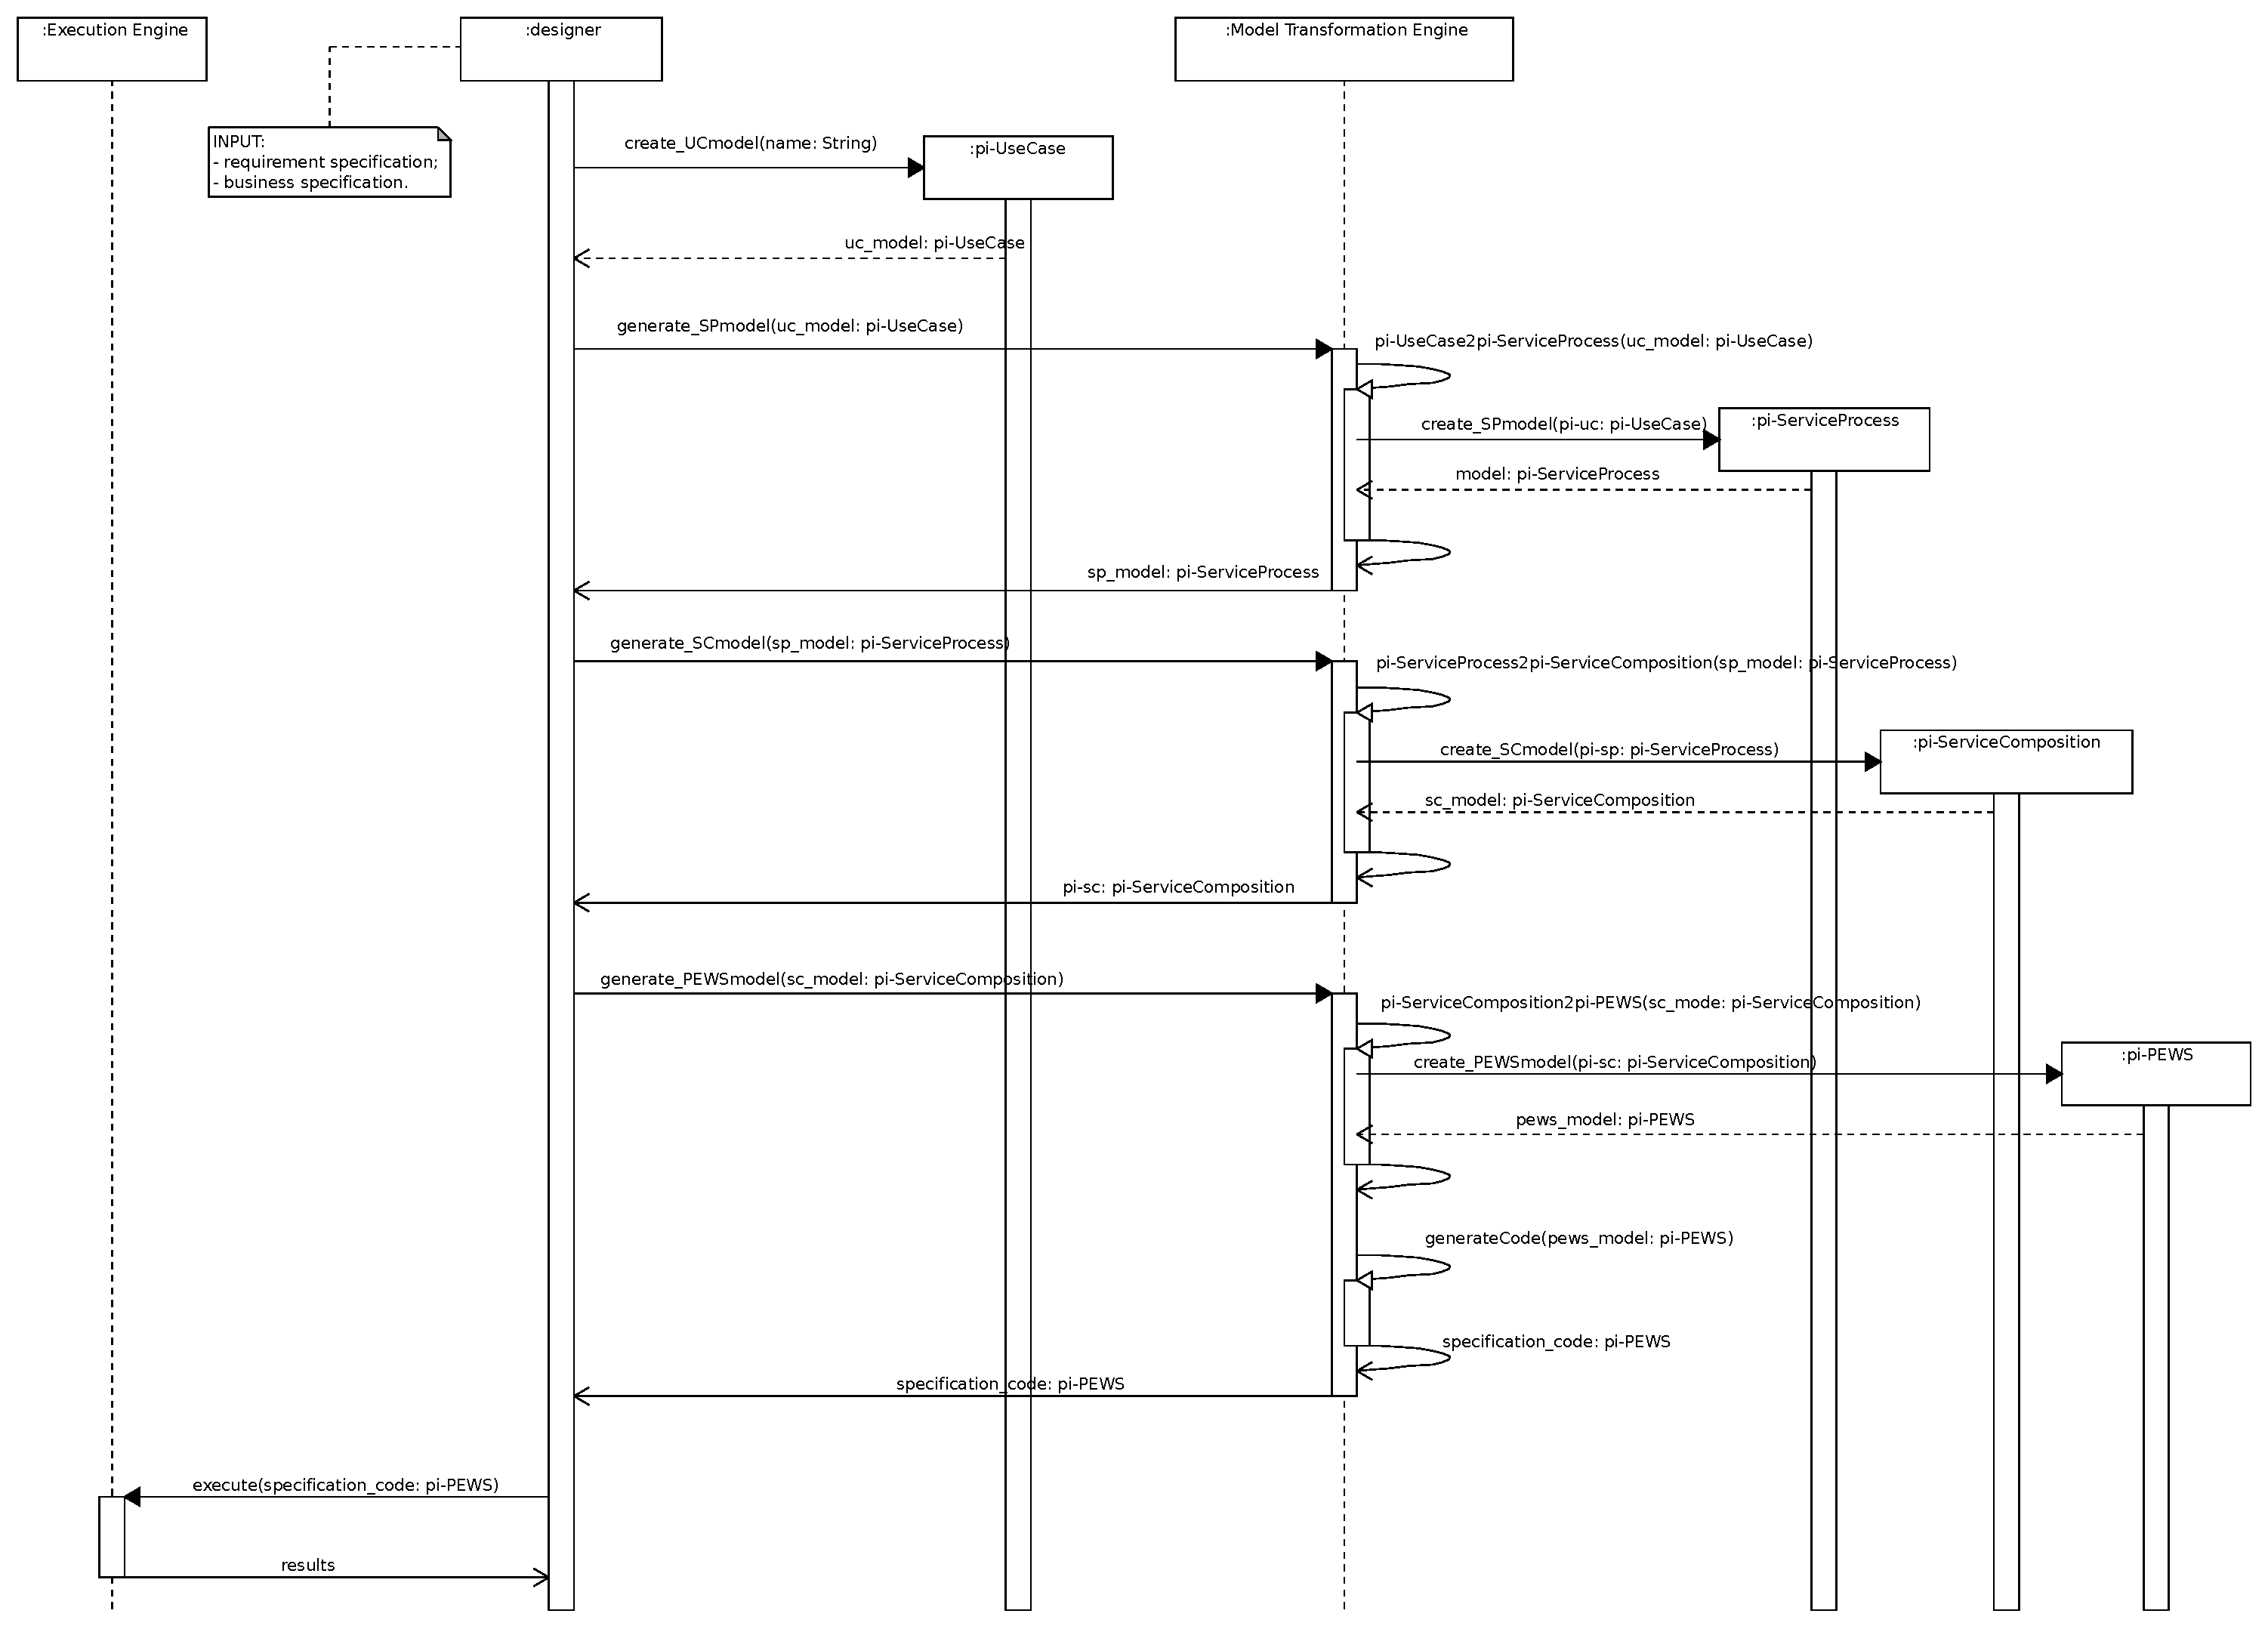
\includegraphics[width=25cm,height=15cm]{chapters/implementation/figs/sequenceDiagram.pdf}
\caption{Model Transformation Process.}
\label{fig:sequenceDiagram}
\end{figure}
\end{landscape}


 
%  The next section will describe how the creation and generation of each model in
%  SOD-M  is done, for better understanding the transformations process
%  represented in figure \ref{fig:sequenceDiagram} .   


\section{Defining Reliable Service Based Applications}
\label{sec:install}

% \footnote{The environment download
% can be performed at http://www3.ifrn.edu.br/\~placido/piSOD-M} 
 
The $\pi$SOD-M environment development
starts with the creation of a project and then the definition of a
\textit{$\pi$-UseCase} model\footnote{To create a model, the user must execute the sequence: \textit{File > New
> Other > EMF Model Wizard}, and choose one of the methodology's model.}, supposing that the business and requirement
specification document have been previously completed.  Figure \ref{fig:screanPiSODM} presents the views provided by the environment:
 \textit{Project view, Menu view, Editor view} and \textit{Properties view}. 



% As $\pi$SOD-M environment is based on Eclipse, the developer and analyst
% need not struggle to adapt to the modeling environment. Figure
% \ref{fig:screanPiSODM} presents a tool overview, which has four views:

 

\begin{figure}[ht!]

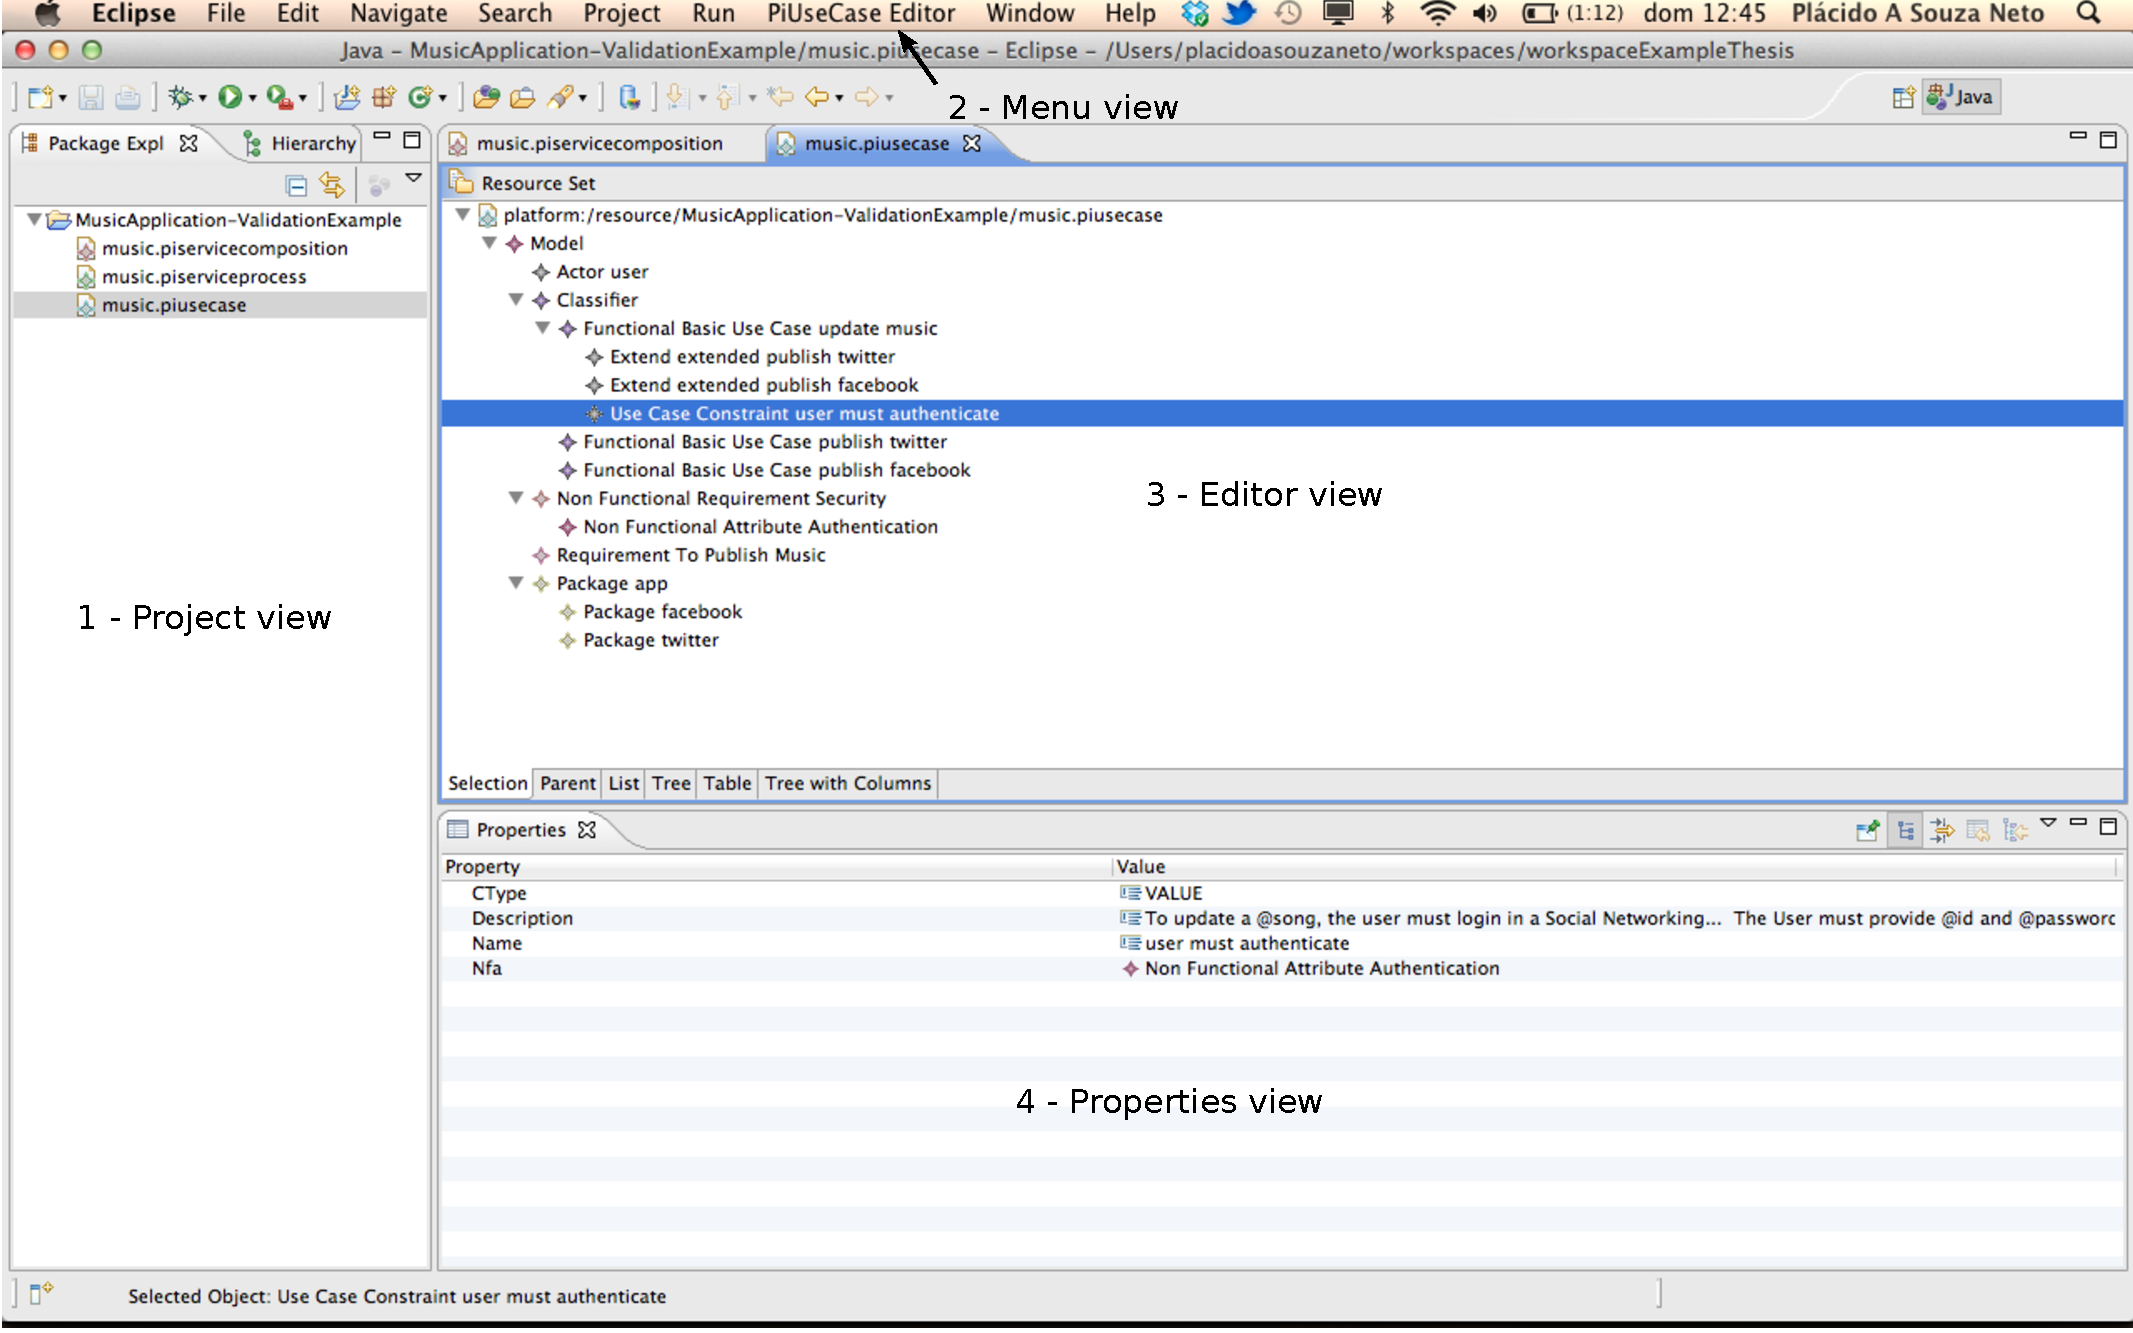
\includegraphics[width=.99\textwidth]{chapters/implementation/figs/telaPiSOD-M.pdf}
\caption{$\pi$SOD-M Eclipse Plugin Environment.}
\label{fig:screanPiSODM}
\end{figure}
 



% For editing is important to follow the concepts presented in $\pi$SOD-M
% meta-models, because it must follow rigorously its structure.

\subsection{\textit{$\pi$-UseCase} Model} 

The goal of creating a \textit{$\pi$-UseCase} is to represent the functions and
system services described in the requirements specification and
business specification documents, which are the requirements input for this
phase. In accordance to the process described in figure \ref{fig:sequenceDiagram}, the designer receives the
documents as input and creates the \textit{$\pi$-UseCase} model. With this
model created, the transformation component generates the
\textit{$\pi$-ServiceProcess} model as output.

 To create the \textit{$\pi$-UseCase} model, it is necessary
choose the root element (\textit{Model}) as the starting point of modeling,
during the process of create a ``\textit{new .piusecase file}'' (
using the sequence, \textit{File > New > Other > EMF Model Wizard}). From
this point the model is created as a tree of elements with its specific
references, as shown in Figure \ref{fig:pisodmToolModel}, which shows the model elements and its equivalence in the graphical $\pi$-UseCase
model, each element is built in an iterative way and must obey the hierarchy
and its relationships.

Each model element has a number of childs or siblings to which it is related to,
\textit{e.g.}, an {\sc Use Case} relates {\sc Constraint}, {\sc Extend} and
{\sc Include} elements, as well as {\sc NFRs} relates {\sc NFAs}.
Figure \ref{fig:pisodmToolModel} shows how to create the model elements for the
``\textit{to publish music}'' scenario.



\begin{figure}[ht!]
\centering
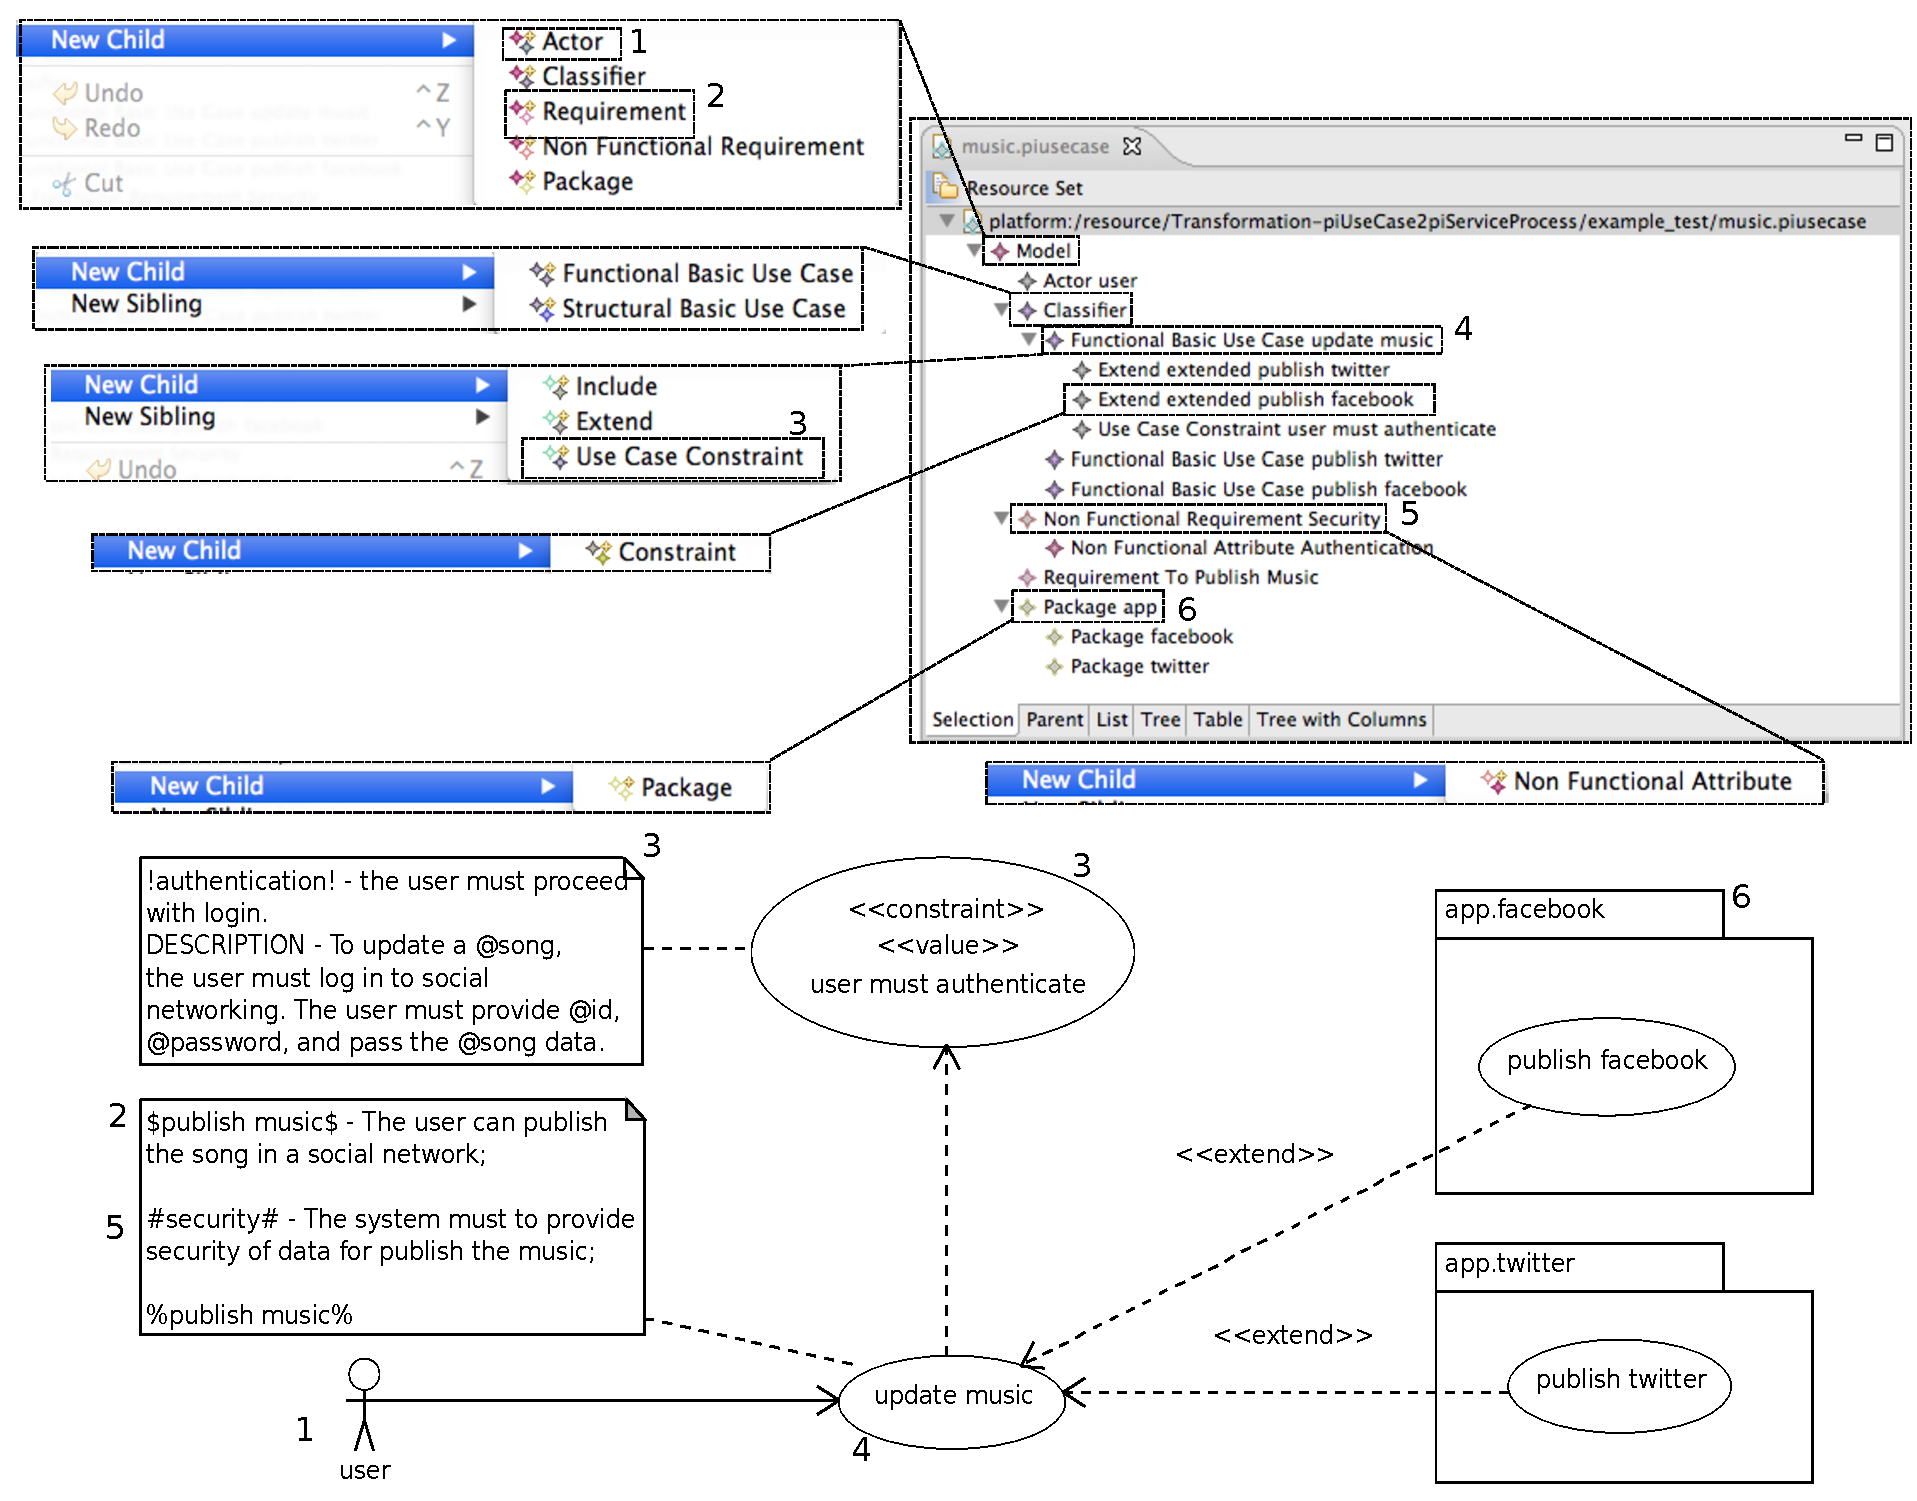
\includegraphics[width=.99\textwidth]{chapters/implementation/figs/create_model-UseCase.pdf}
\caption{$\pi$-UseCase Model Definition in $\pi$SOD-M Eclipse Plugin.}
\label{fig:pisodmToolModel}
\end{figure}


\begin{exampl}
Items 1 and 2 in Figure \ref{fig:pisodmToolModel} show how to create an
{\sc Actor} and a {\sc Requirement}, item 3 presents the \textit{update music}
{\sc Use Case} and how to create a {\sc Constraint} related to this element.
Item 4 makes reference to a {\sc Constraint} and finally, the items 5 and 6 are
equivalent to a {\sc NFR} and a {\sc Package} elements, respectively. Each item
in the model refers to a equivalent element in the graphical model.
\end{exampl}

Figure \ref{fig:pisodmToolModelProperties} presents some configuration
properties. After creating an element, it is necessary to set its properties.
All elements have properties that describes their relationship and specification
values. These properties are used to give specification details, as
well as future transformations. 

% All properties must be set, except of the
% properties are not used in the specification of one specific application, for
% example, there is no exceptional behaviour for an action. In this case it is not
% necessary to set this property. Another example that is no necessary set a
% element property is an actor or use case are not related with a package.

\begin{exampl}
Item 1 in Figure \ref{fig:pisodmToolModelProperties} shows the {\sc Use Case}
element properties for the ``\textit{to publish music}'' application. After the
creation of a use case it is necessary to create the actor, its \textit{name}, which \textit{requirement} the \textit{use case}
belongs, and the respective \textit{package}. Item 2 shows the properties of a {\sc Constraint} element. In a
constraint, its type must be explicit (\textit{VALUE, BUSINESS} or
\textit{EXCEPTIONALBEHAVIOUR}), its \textit{description}, with all candidate
\textit{variables} described with an `\textit{@}', its \textit{name} and which
{\sc Non-Functional Attributes} element this constraint is related to,
\textit{e.g.}, \textit{Authentication}, is an attribute of the
{\sc Non-Functional Requirements}, \textit{Security}. Items 3 and 4 show the
 ``\textit{To Publish Music}'' requirement properties and package
``\textit{app}'', respectively. The properties of each element obey the elements
described in the \textit{$\pi$-UseCase} meta-model. 


\end{exampl}


\begin{figure}[ht!]
\centering
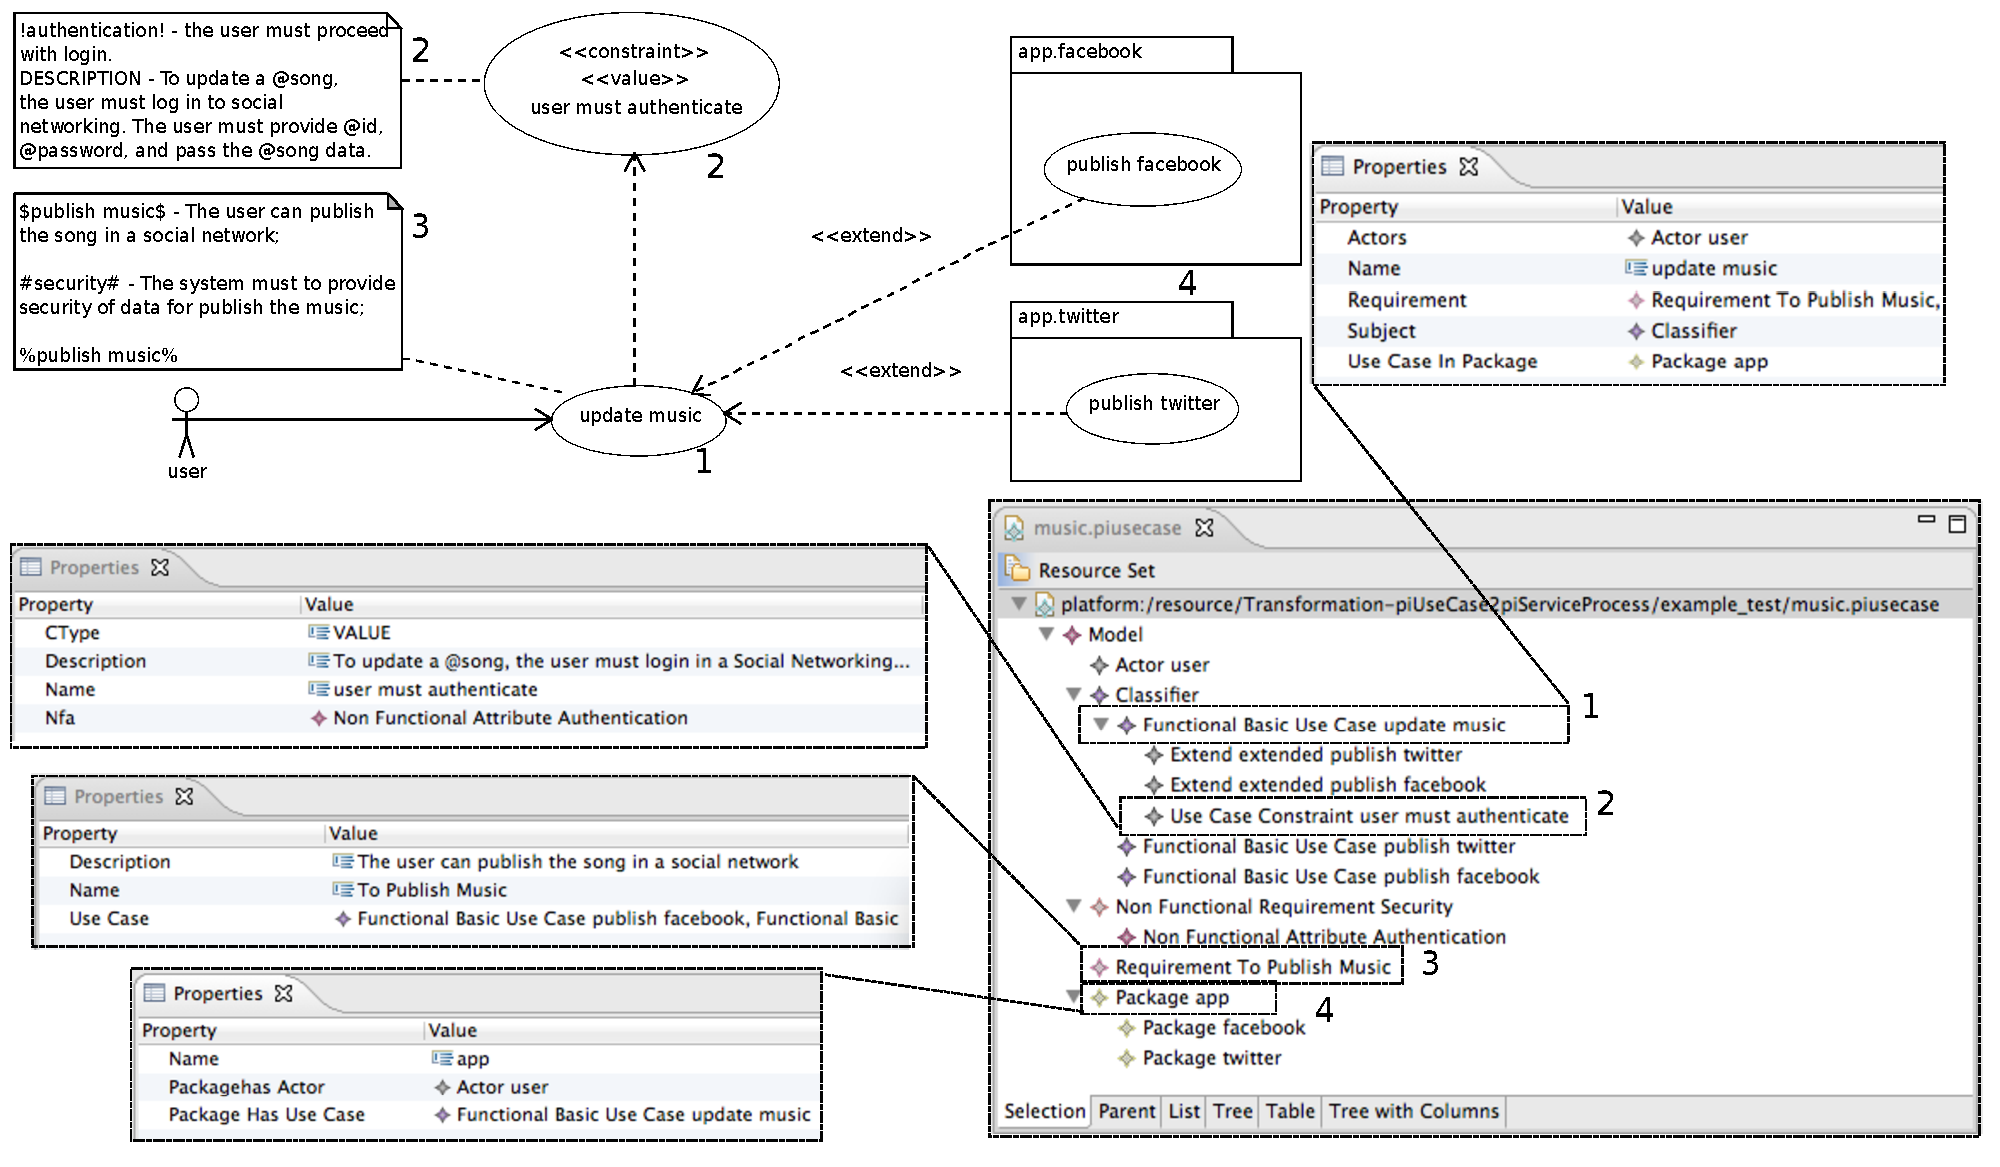
\includegraphics[width=.99\textwidth]{chapters/implementation/figs/model-UseCase.pdf}
\caption{\textit{$\pi$-UseCase} Properties in $\pi$SOD-M Eclipse Plugin.}
\label{fig:pisodmToolModelProperties}
\end{figure}


\subsection{\textit{$\pi$-ServiceProcess} Models}

The goal of creating a \textit{$\pi$-ServiceProcess} model is to represent the
system execution flow. The designer receives the
\textit{$\pi$-UseCase} model as input to generate the
\textit{$\pi$-ServiceProcess} model. After the \textit{$\pi$-ServiceProcess}
model be generated, the designer calls again the model transformation component
to generate the \textit{$\pi$-ServiceComposition} model as output (figure
\ref{fig:sequenceDiagram}).

 To create the \textit{$\pi$-ServiceProcess} model, it is necessary
choose the root object (\textit{Service Process}) as the starting point of
modeling, during the process of create a ``\textit{new .piserviceprocess file}''
option. From this point on, the model is created as a tree with its specific
references.

%  Figure \ref{fig:piserviceProcessToolModel} 
% presents the service process model, a graphical model reference and detail of
% how create each model element. It is possible to create the $\pi$-ServiceProcess
% model in isolation, however this model is generated from the previous model
% descriptions.

As this model is a refinement of the concepts described in the previous model,
its information is part of the information and properties of the
\textit{$\pi$-UseCase} model, but they focus on the process workflow
and application functions. 

\begin{exampl}
Figure \ref{fig:piserviceProcessToolModel} shows the complete model of the example scenario and its main components. From
the root element the user can create the following elements: {\sc Service
Activity, Object Flow, Control Flow, Contract} and {\sc Non-Functional
Attribute}. In Figure \ref{fig:piserviceProcessToolModel}, item marked with 1
highlights the creation of the {\sc Control Flow }. Items 2 and 3 show the elements {\sc Fork
Node} and {\sc Join Node}, respectively, essential for the execution flow
description. Items 4 show the {\sc Action} element, which describes the
\textit{download music, listen music} and \textit{publish twitter} actions and
finally, items 5 highlight the {\sc Assertion} element, which is used to
describe the restrictions over each {\sc Action}.   
\end{exampl}

 
\begin{figure}[ht!]
\centering
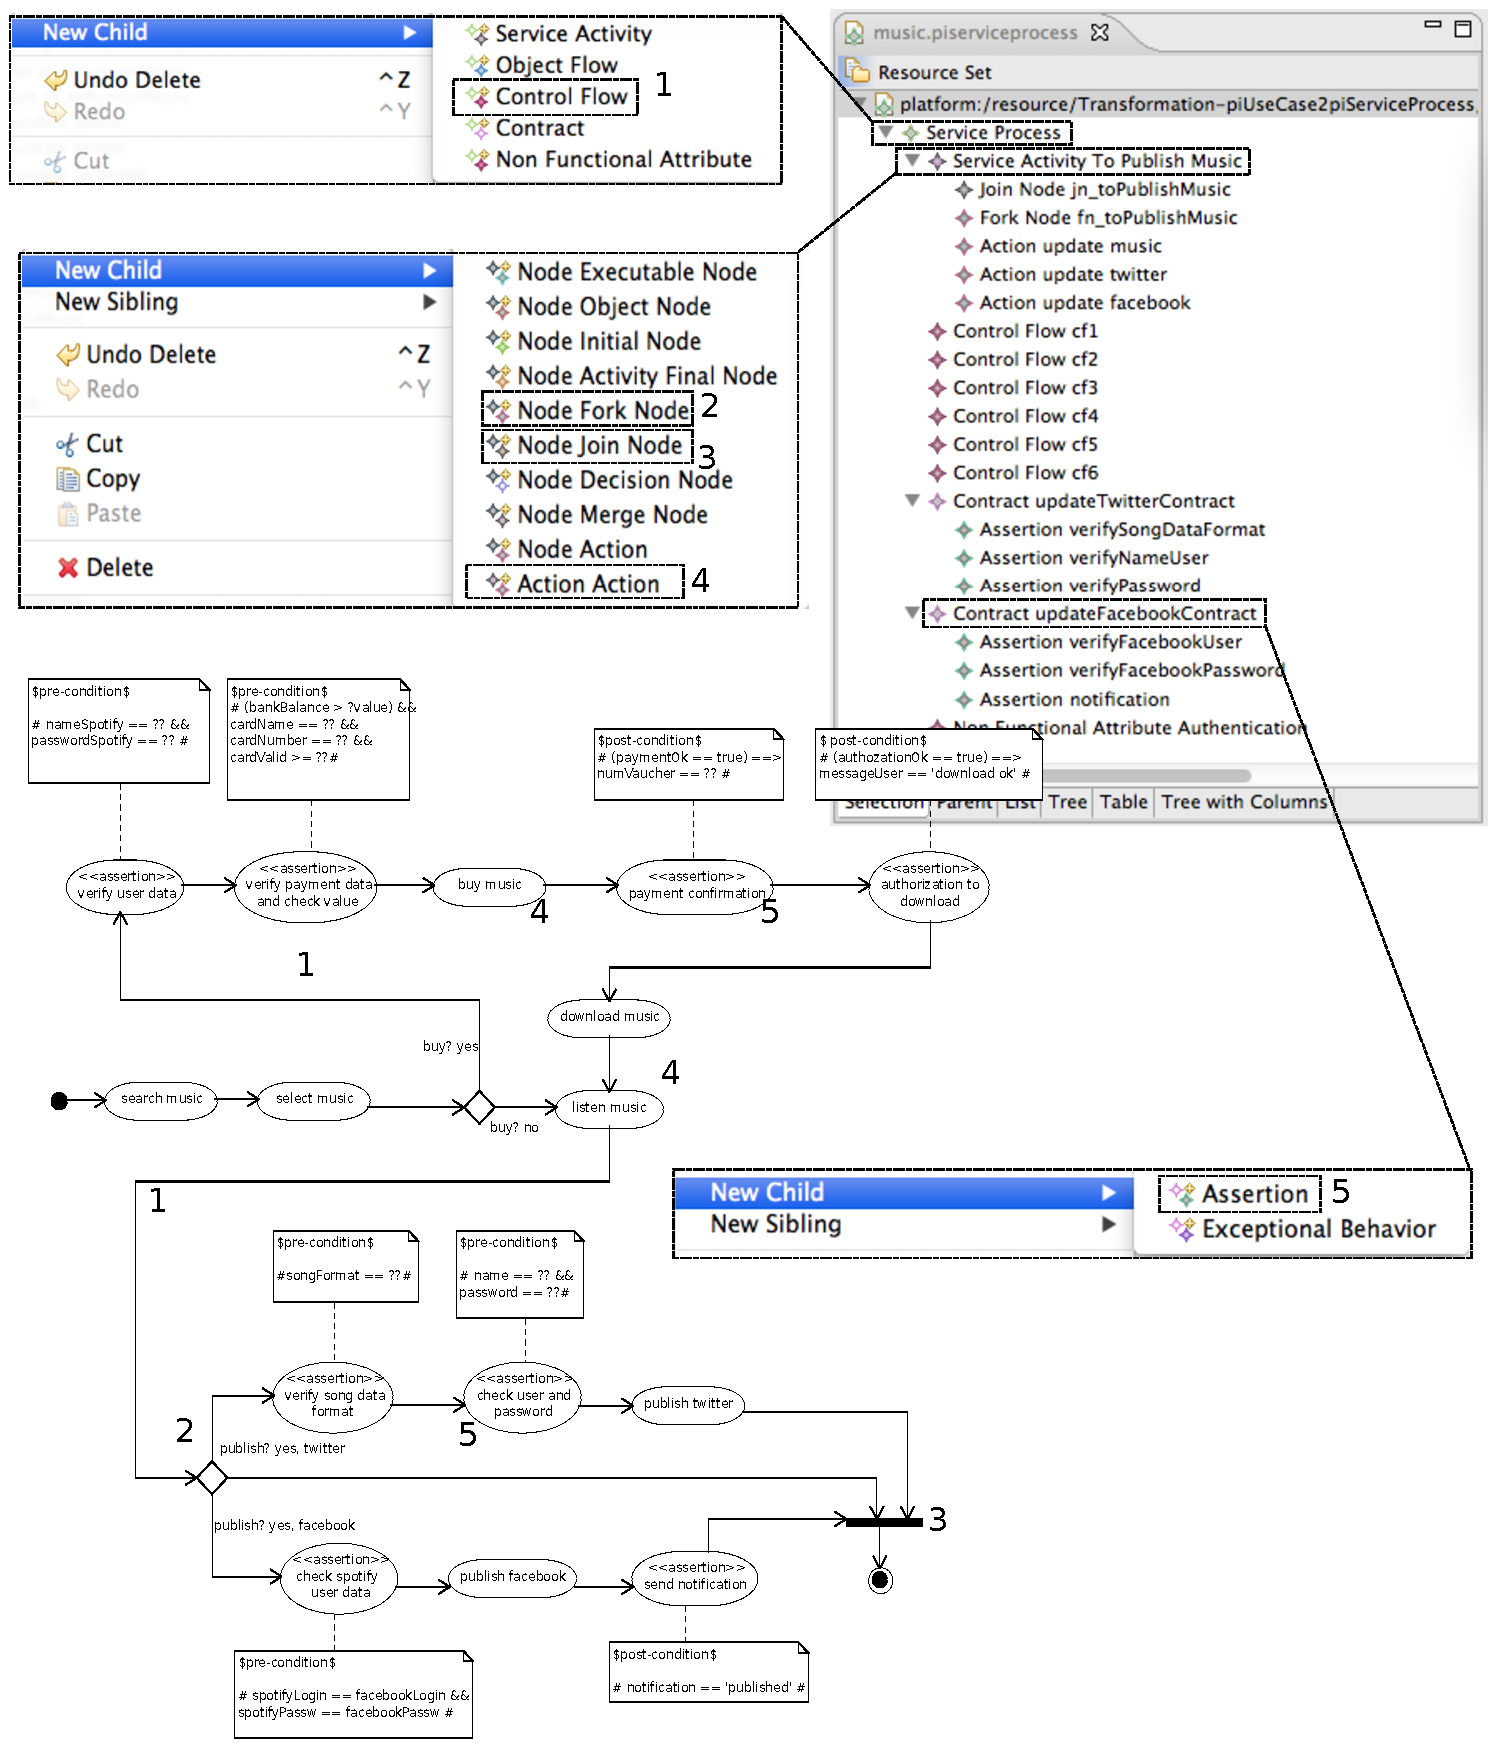
\includegraphics[width=.99\textwidth]{chapters/implementation/figs/create_model-ServiceProcess.pdf}
\caption{\textit{$\pi$-ServiceProcess} Model Definition in $\pi$SOD-M Eclipse
Plugin.}
\label{fig:piserviceProcessToolModel}
\end{figure} 

The designer must also configure the properties of each
\textit{$\pi$-ServiceProcess} model element to complete it by specifying all
constraints that compose the contracts and the application process. Figure
\ref{fig:piserviceProcessToolModelProperties} presents the properties of the
main model elements for our example scenario. These properties complement the
modeling of the execution flow.
   
\begin{figure}[ht!]
\centering
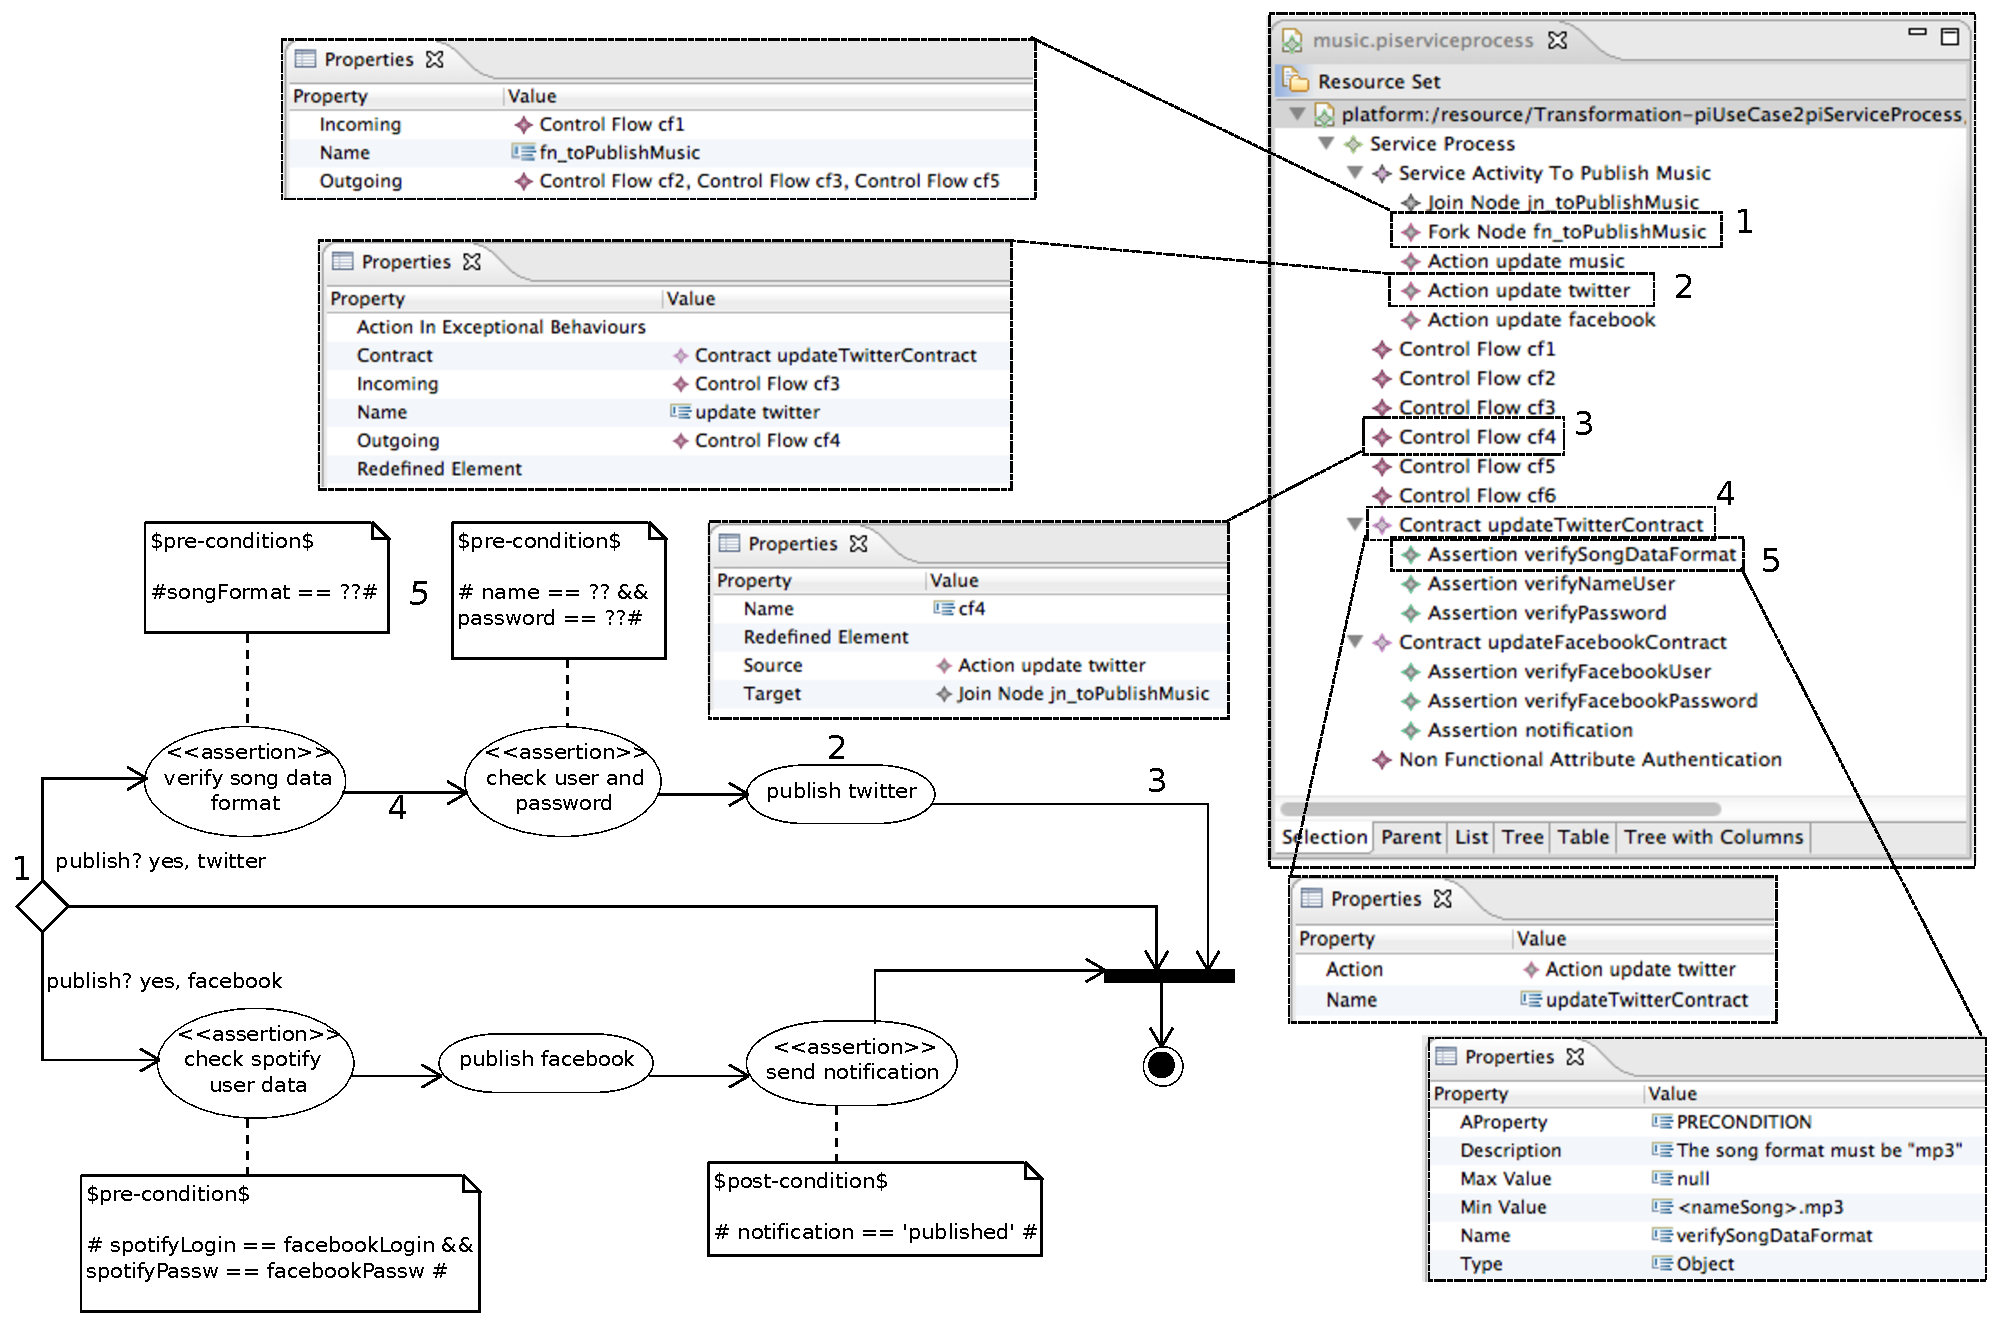
\includegraphics[width=.99\textwidth]{chapters/implementation/figs/model-ServiceProcess.pdf}
\caption{\textit{$\pi$-ServiceProcess} Properties in $\pi$SOD-M Eclipse Plugin.}
\label{fig:piserviceProcessToolModelProperties}
\end{figure} 


\begin{exampl}
Items 1 in Figure \ref{fig:piserviceProcessToolModelProperties}
describe the properties of a {\sc Fork Node}, which is associated with {\sc Edge Activities}
({\sc Control Flow} and {\sc Object Flow}) that connect the {\sc Action}
elements. For example, the {\sc Fork Node} \textit{fn\_toPublishMusic} has an
input edge (\textit{cf1}) and three output streams edges (\textit{cf2, cf3} and
\textit{cf5}). All these elements are {\sc Control Flow} entities (items 3).
Items 2 show the {\sc Action} properties, and items 4 and 5 describe a {\sc
Contract} and its {\sc Assertions} properties, respectively. A {\sc Contract}
has a \textit{name} and the information of an {\sc Action}.
{\sc Assertions} are {\sc Contract}'s child element. Each  {\sc Contract} can
have many  {\sc Assertions}. Each  {\sc Assertion} has six properties, they are:
(i) \textit{AProperty}, which describes the runtime verification execution time,
(ii) \textit{description}, (iii) \textit{variable name}, (iv and v) a maximum
and minimum allowed to be checked (\textit{MaxValue} and \textit{MinValue}) and
the variable (vi) \textit{type}. In cases of non numeric types, \textit{e.g.}
\textit{Short Int, Flot} and \textit{Double}, only \textit{MinValue} property
value is considered property  and\textit{MaxValue} is described as
\textit{null}.
\end{exampl}
 
\subsection{\textit{$\pi$-ServiceComposition} Models}

The goal of creating a \textit{$\pi$-ServiceComposition} model is to represent
the system service compositions and to reference the external services
that are called by the application. The designer receives the
\textit{$\pi$-ServiceProcess} model as input to generate the
\textit{$\pi$-ServiceComposition} model. After the
\textit{$\pi$-ServiceComposition} model is generated, the designer calls again
the model transformation component to generate the \textit{$\pi$-PEWS} model as
output (figure \ref{fig:sequenceDiagram}). The output model describes the system
specification in a specific platform. 

To create the \textit{$\pi$-ServiceComposition} model, it is necessary to choose
the root object (\textit{Composition Service Model}) as the starting point of modeling,
during the process of creating a ``new .piservicecomposition file'' option. From
this point on, the model is created as a tree with its specific references.

Recall that the \textit{$\pi$-ServiceComposition} model is a refinement of
\textit{$\pi$-ServiceProcess} model, most elements are the same, except for {\sc
Business Collaborator, Policy, Rules} and {\sc Variable}. Thus, we will detail these elements in the
model editor description. 

\begin{exampl}
Figure \ref{fig:piserviceCompositionToolModel} shows
the relationship of these elements for our example scenario. Each {\sc Action}
has an specific {\sc Business Collaborator} (item 3), this elements express the external service
provider, such as Facebook, Twitter or Bank. Another example of a {\sc Business
Collaborator} definition is a WSDL specification. The WSDL namespaces represents
a kind of {\sc Business Collaborator}. Besides {\sc Business Collaborator}
element, the main children root element (\textit{Composition Service Model})
are: {\sc Policy} and {\sc Service Activity} (items 1), and each {\sc Policy}
(items 2) is directly related with {\sc Service Activities}. From a {\sc Policy}
it is possible to create a set of {\sc Rules} (item 4). Figure
\ref{fig:piserviceCompositionToolModel} also presents an equivalent graphic
model of the application. In this figure, the \textit{Application}'s {\sc
Business Collaborator} presents only the main {\sc Actions} (\textit{buy music, listen music, publish
Facebook} and \textit{publish twitter}) that are related with a {\sc Service
Activities} that have one {\sc Policy}. The \textit{Application}'s {\sc Business
Collaborator} model is the same presented in the previous section
(\textit{$\pi$-ServiceProcess} model).

\end{exampl}

 
  
\begin{figure}[ht!]
\centering
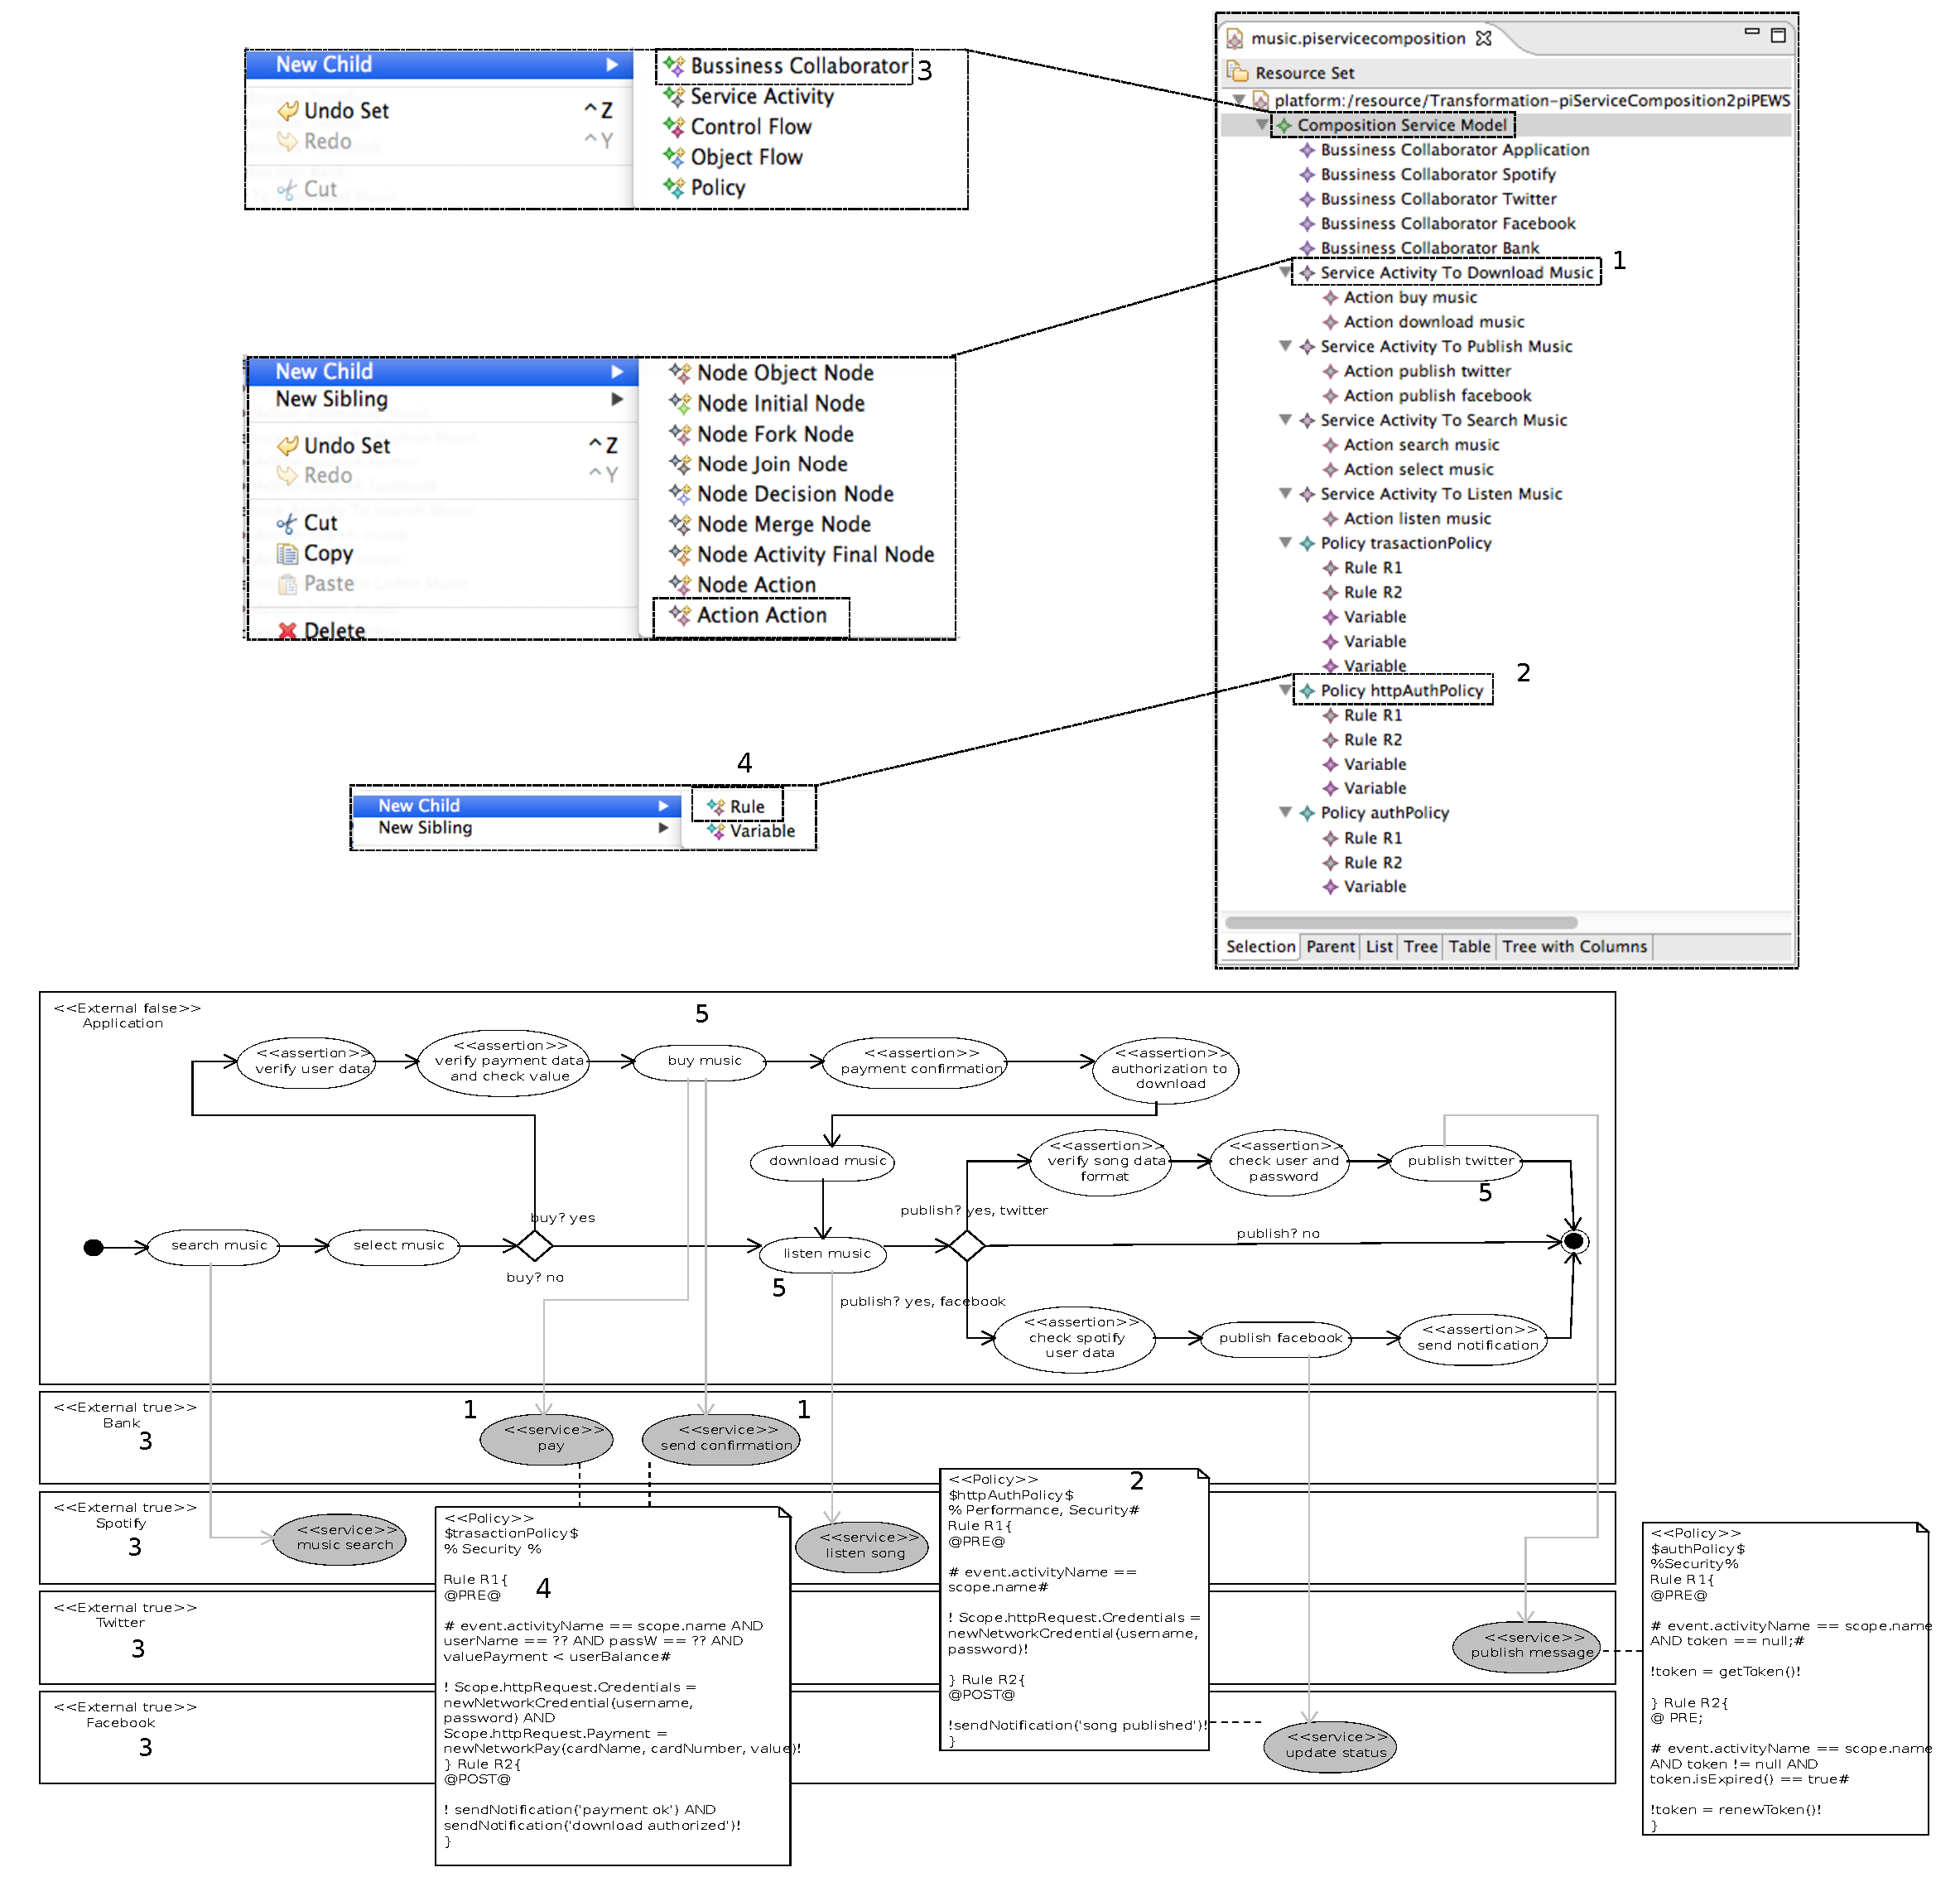
\includegraphics[width=.99\textwidth]{chapters/implementation/figs/create-model-Serviceconposition.pdf}
\caption{\textit{$\pi$-ServiceComposition} Model Definition in $\pi$SOD-M
Eclipse Plugin.}
\label{fig:piserviceCompositionToolModel}
\end{figure}

The properties of \textit{$\pi$-ServiceComposition} elements are
configured as the same way the other two previous editors, and the properties
described in the \textit{$\pi$-ServiceComposition} meta-model
(Figure \ref{fig:servicecomposition}). Thus, to configure the properties of this model,
it is necessary simply choose the desired element and to modify its values.


\subsection{\textit{$\pi$-PEWS} Models}

The goal of creating a \textit{$\pi$-PEWS} model is to represent
the application in a specific platform. The designer receives the
\textit{$\pi$-ServiceComposition} model as input to generate the
\textit{$\pi$-PEWS} model. After the
\textit{$\pi$-PEWS} model be generated, the designer calls again
the model transformation component to generate the \textit{$\pi$-PEWS}
specification code as output (figure \ref{fig:sequenceDiagram}). This code will
be executed. 
 
To create the \textit{$\pi$-PEWS} model, it is necessary to choose the root
object (\textit{PEWS Spec}) as the starting point of modeling. From
this point on, the model is created as a tree with its specific references.

The \textit{$\pi$-PEWS} meta-model is a representation of the
\textit{$\pi$-PEWS} language. Each \textit{$\pi$-PEWS} model is a
program/specification written in that language. The elements described in this
model represent parts of language's grammar constructs. Each entity in the model
represents a piece of \textit{$\pi$-PEWS} code.
	
\begin{figure}[ht!]
\centering
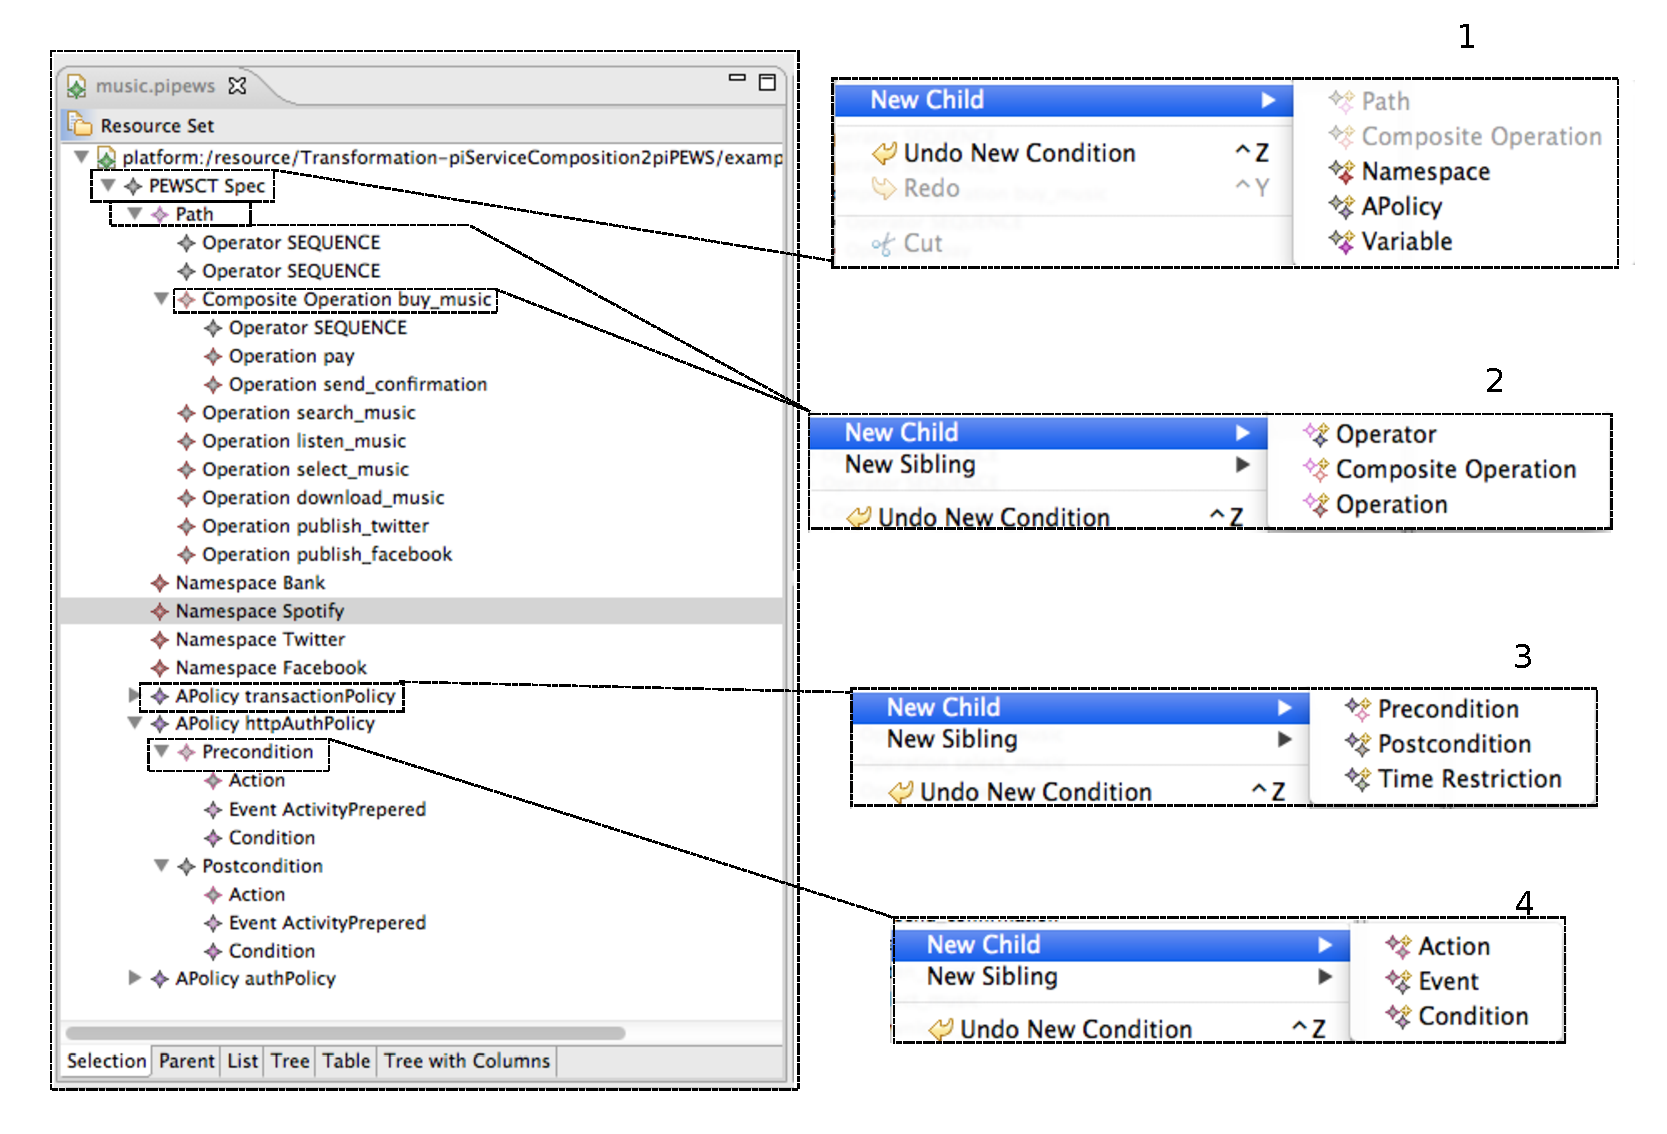
\includegraphics[width=.90\textwidth]{chapters/implementation/figs/create_model-PEWS.pdf}
\caption{\textit{$\pi$-PEWS} Model Definition in $\pi$SOD-M Eclipse Plugin.} 
\label{fig:piPEWSToolModel}
\end{figure}

Figures \ref{fig:piPEWSToolModel} and \ref{fig:piPEWSToolModelProperties}
show how the elements that compose a \textit{$\pi$-PEWS} model can be specified
in our tool. This model is generated automatically from the
\textit{$\pi$-ServiceComposition} model.      

\begin{figure}[ht!]
\centering
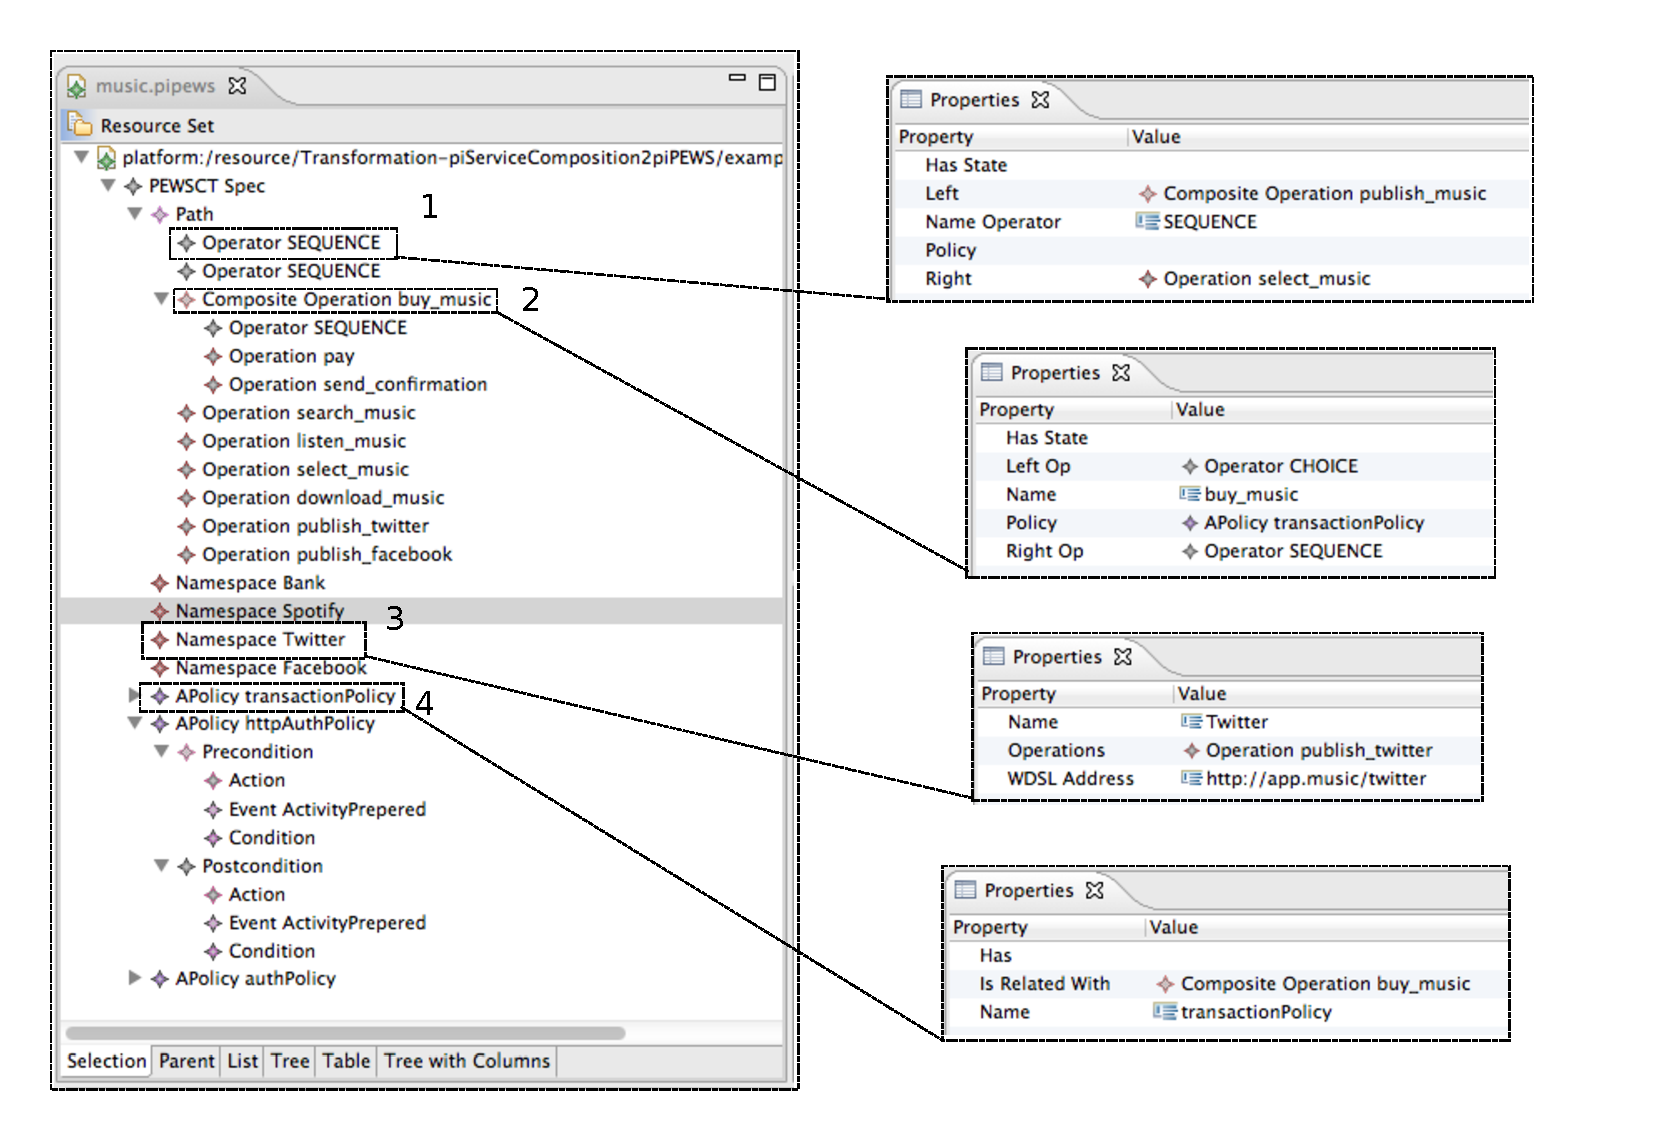
\includegraphics[width=.90\textwidth]{chapters/implementation/figs/create_model-PEWSProperties.pdf}
\caption{\textit{$\pi$-PEWS} Model Properties in $\pi$SOD-M Eclipse Plugin.} 
\label{fig:piPEWSToolModelProperties}
\end{figure}


\textit{$\pi$-PEWS} is the last model generated before the code generation. At
this stage, it is spected that the designer proceeds with a general (manual)
check of consistency of the model. It is
important to remark that the environment alone does not replace the
modeling work required to design and develop services based applications. 

\section{Extending the Environment} 
\label{sec:extendingEnvironment}

Both, the $\pi$SOD-M environment and methodology can be extended, in order
to improve the components that describe and implement the methodology.
Extensions can be done in two different levels: (i) adding new models to the
existing infra-structure, and (ii) considering more abstract levels.

The extension may be in terms of language: new meta-models for other
languages can be described and coupled to the environment. The extension process
should take place as follows: new languages meta-models may be designed and
coupled in the environment architecture (such as BPEL, XAML, WSDL and XLANG).
After creating the desired meta-model, a mapping must be done. The mapping must
respect the \textit{$\pi$-ServiceComposition} meta-model. It is also necessary
to describe the rules for code generation, using a code generator engine such
Acceleo.

% Thus, new
% languages may be added for the environment improvements and for improve the
% methodology flexibility. 

Considering the more abstract level of the methodology, new
meta-models can be described. For instance, the computing independent level
(CIM level) of SOD-M may be added to our methodology to describe the
requirements and business restrictions in terms of models. 


% \begin{figure}[ht!]
% \centering
% 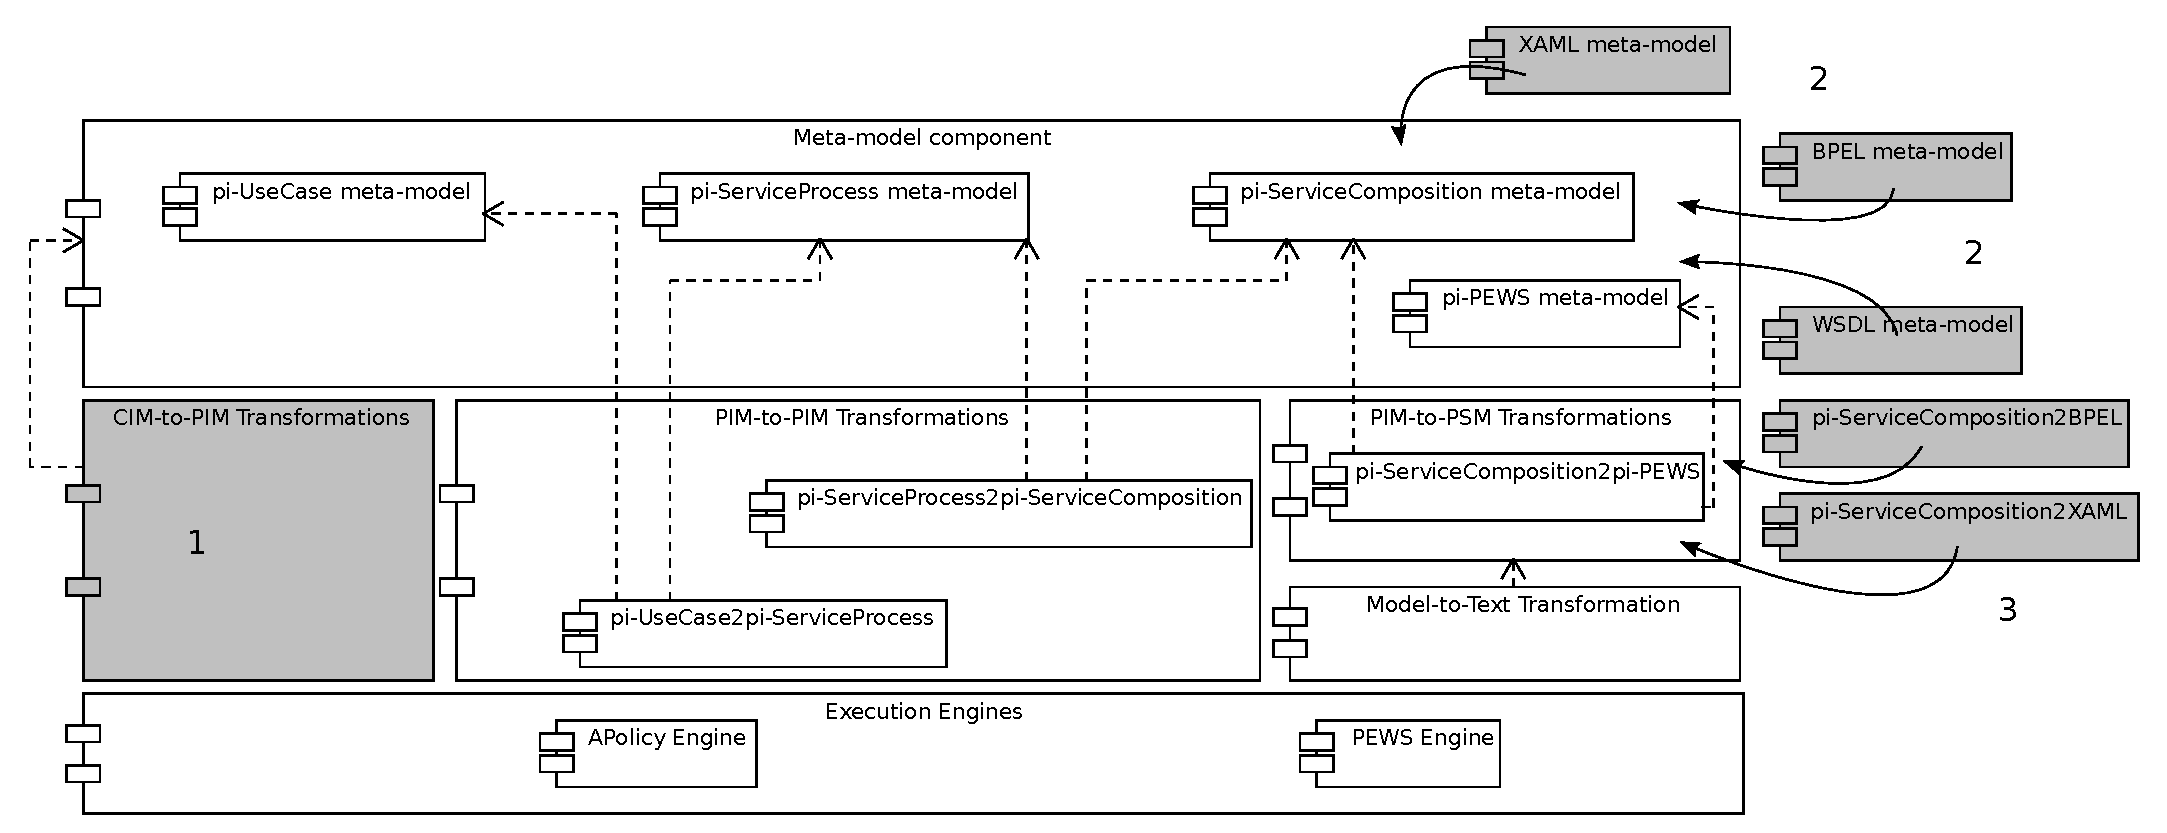
\includegraphics[width=.95\textwidth]{chapters/implementation/figs/componentes.pdf}
% \caption{$\pi$SOD-M Environment Extension Components.}
% \label{fig:extension}
% \end{figure}
% 
% 
%  
% 
% Figure \ref{fig:extension} presents how the environment can be extended.
% The components that can be inserted components of CIM-to-PIM transformation
% models (item 1), new languages meta-models description (item 2) and
% components which represent the transformations between the
% \textit{$\pi$-ServiceComposition} model and each language (item 3). Thus, it is
% possible to extend the development environment of SOD-M. The extension must comply with
% the methodology concepts and environment architecture.     
 
\section{Conclusion} 
\label{sec:env_conclusion}

This chapter introduced the implementation
 of the $\pi$SOD-M methodology environment. We also presented a representation
 for our model description. The implementation includes all (i) meta-models of
 $\pi$SOD-M, (ii) editors for each model for the applications being developed,
 and (iii) the plugins for the transformations defined by the methodology. An
 example was also presented to describe the environment features.
  
 
%  This graphical representation can be better refined
%  in future work, focussing on processing models or on the development of a
%  visual tool for processing models and code generation.

% It was
% presented and described the general environment architecture, its properties, language used, its execution environment and how to extends the environment. The
% development environment of $\pi$SOD-M supports the methodology for a better use of their concept. 

 

% Using the proposed graphical nomenclature, we described all the transformation
% rules that were used for the development of the environment's plugin responsible
% for the transformation of all $\pi$SOD-M models. This chapter also presented, in
% detail, all $\pi$SOD-M meta-models and editors, such as how to extend the
% environment and use it. Finally, after the design description, were
% introduced the execution environment example for the development each models in
% $\pi$SOD-M context.
    